\documentclass{article}
\usepackage{graphicx} % Required for figures
\usepackage[numbers]{natbib}
\usepackage{float} % Add this in your preamble
\usepackage{amsmath}
\usepackage{amsfonts}
\usepackage[utf8]{inputenc}
\usepackage{hyperref}




\title{paper collagen}
\author{robert.tavares}
\date{November 2023}

\begin{document}

\maketitle

\section{Introduction}

    O colágeno tipo I, que constitui $90\%$ da matriz extracelular humana, é caracterizado por sua estrutura de tripla hélice 
    polipeptídica ($\alpha$-cadeias), com dimensões típicas de $300$ nm de comprimento e $1,5$ nm de diâmetro, assemelhando-se 
    a hastes \cite{Gelse2003,Silver2018}. Intrinsecamente programadas para a auto-organização, as moléculas de colágeno se 
    agregam em estruturas fibrilares durante a fibrilogênese, alinhando-se em intervalos de $D=67$ nm, permitindo cinco 
    configurações de interação \cite{Zhu2018, KADLER1996}. 
    
    As fibrilas de colágeno exibem uma forma alongada, caracterizada por uma região central densa e extremidades afiladas, 
    com comprimentos típicos em torno de \(500 \mu m\) e diâmetro de \(500 nm\), sendo compostas por cerca de \(10^{7}\) moléculas 
    \cite{Charvolin2019, KADLER1996, Parry1984}. A agregação dessas fibrilas forma fibras de colágeno, com diâmetros aproximados 
    de \(20 \mu m\), que servem como pilares para estruturas hierárquicas mais complexas e variadas, incluindo tecido conjuntivo, 
    ossos, tendões e córnea \cite{RicoLlanos2021}. A presença de colágeno nessas estruturas é fundamental para suas propriedades 
    elásticas e mecânicas \cite{Silver2018}. 

    A relevância das fibras de colágeno se torna evidente ao compreendermos seu papel essencial no corpo humano. A jornada para 
    desvendar esses mistérios é longa e esbarra em um desafio significativo: a minúscula escala das fibrilas. Esta escala nanométrica 
    impõe dificuldades na investigação de suas propriedades mecânicas, exigindo equipamentos de precisão nanométrica para tais análises 
    \cite{Nalbach2022InstrumentFT}. Entre as técnicas empregadas, a Microscopia de Força Atômica (AFM) destaca-se por sua aplicabilidade
    frequente no estudo detalhado das fibrilas de colágeno, com um foco particular na análise de sua estrutura 
    \cite{Andriotis2015-lx,Mull2022-br}. Pioneiramente, Van der Rijt e colaboradores \cite{Rijt} utilizaram a AFM para avaliar as 
    propriedades mecânicas de fibrilas de tendão isoladas, elucidando seu comportamento sob tensão até o ponto de falha. 

    A literatura evidencia uma diversidade de modelos computacionais dedicados ao estudo das fibrilas de colágeno e suas características 
    mecânicas. Notavelmente, Buehler e seus colaboradores introduziram uma metodologia baseada em granulação grossa e dinâmica molecular, 
    que elucida profundamente a arquitetura e o comportamento das fibrilas sob tensões ou em processos de degradação, e examina o efeito 
    de componentes minerais incorporados \cite{B1,B2,B3,B4,Malaspina2017-qp,10.1002/jbmr.2705}. Alternativamente, uma abordagem fundamentada 
    em primeiros princípios emprega osciladores harmônicos, analogamente a molas, para simular a natureza elástica das fibrilas. Este modelo, 
    aplicado em uma configuração bidimensional, foi explorado por Araujo e equipe para investigar as alterações nas propriedades mecânicas 
    de tecidos sob influência de agentes degradativos \cite{Araujo}. Tal estratégia simplificada facilita o exame de estruturas nanoscópicas 
    e a compreensão do comportamento microscópico do colágeno, minimizando a exigência de recursos computacionais. 

    Em nossa pesquisa, adotamos um modelo de Agregação Limitada por Difusão (\textit{Diffusion Limited Aggregation} - DLA) para simular 
    agregados com morfologias análogas às fibrilas de colágeno \cite{Parkinson1995}. Essas estruturas foram analisadas por meio de um modelo 
    mecânico probabilístico \cite{Parkinson1997}, permitindo-nos investigar seu comportamento sob tensão e examinar o impacto de diferentes 
    parâmetros do modelo na resistência do material. Identificamos a ocorrência de avalanches durante o processo de ruptura, caracterizadas 
    por leis de escala precisas. Acreditamos que essa abordagem integrada, que combina simulação da formação com análise mecânica, possa 
    oferecer perspectivas valiosas sobre as fibrilas de colágeno, possibilitando a exploração de sua estrutura em diferentes estágios. 


\section{Metodologia}

    No presente estudo, desenvolvemos a investigação em duas etapas principais: na primeira, usamos um modelo para a formação de 
    fibrilas de colágeno para estudar sua estrutura; na segunda, analisamos as propriedades mecânicas desses agregados. 

    \subsection{Estrutura das fibrilas}

    Utilizamos um modelo baseado em Agregação Limitada por Difusão (\textit{Diffusion Limited Aggregation} - DLA) \cite{Witten1983} 
    em três dimensões para simular a formação de fibrilas de colágeno. Consideramos as moléculas de colágeno como paralelepípedos 
    regulares de dimensões \(1 \times 18 \times 1\). Empregando uma rede regular cúbica, definimos o centro como a origem e fixamos 
    a primeira molécula do agregado, denominada \textit{seed}. Em seguida, novas moléculas são lançadas a partir de uma distância 
    \(R\) do centro do agregado e se difundem até que ocorra uma das seguintes situações: serem capturadas pelo agregado ou atingirem 
    uma distância \(2R\) em relação ao centro, caso em que a simulação é reiniciada. Esse processo está esquematizado na Figura \ref{M1}. 

        \begin{figure}[H]
            \centering
            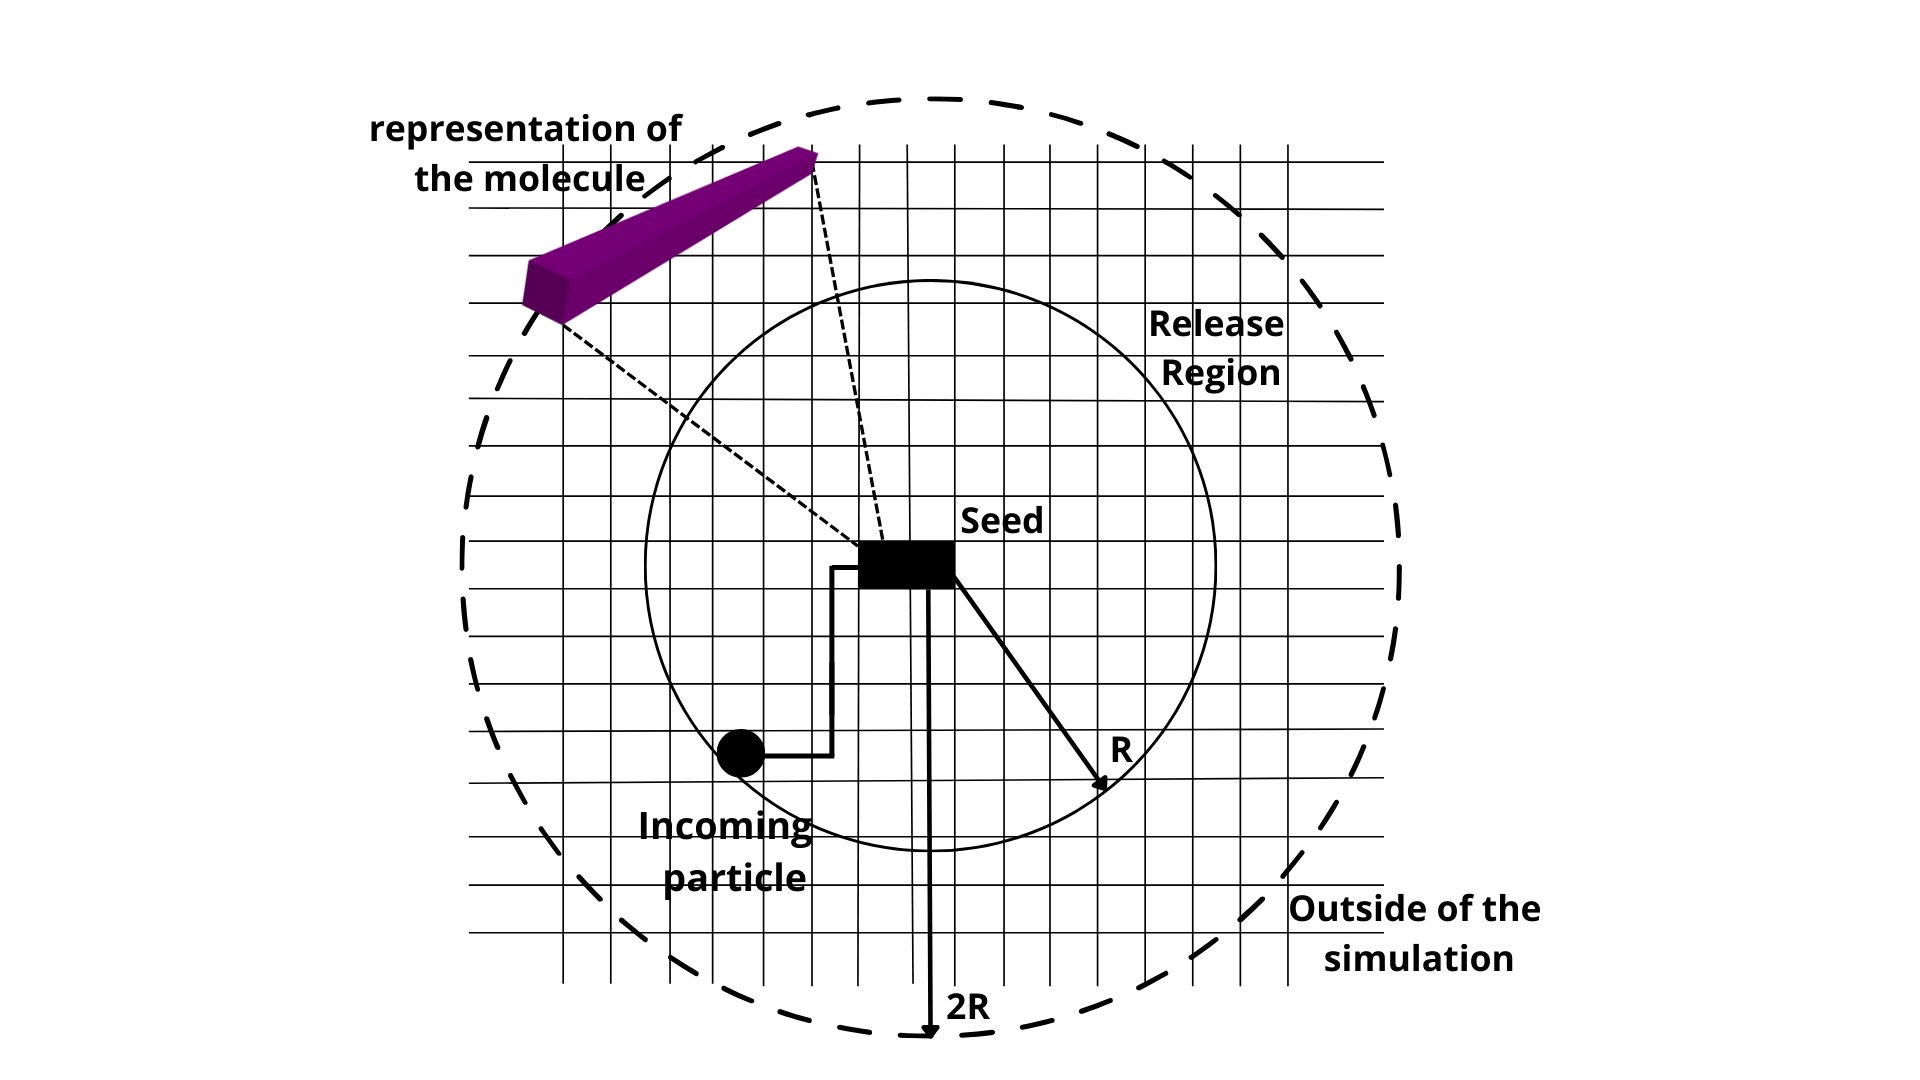
\includegraphics[width=\textwidth]{figures/DLA.png}
    
            \caption{Consideramos as moléculas de colágeno como paralelepípedos regulares de dimensões \(1 \times 18 \times 1\). 
            Estas moléculas são lançadas a partir de uma distância \(R\) da \textit{seed}, que representa a primeira molécula fixada 
            no agregado. As moléculas podem se difundir até serem capturadas pelo agregado ou atingirem uma distância \(2R\) da \textit{seed}, 
            fora da zona de interesse, o que leva à reinicialização da simulação.} 
    
            \label{M1}
        \end{figure}
    
        O processo de difusão das moléculas é modelado por um \textit{random walk} tridimensional, permitindo movimentos para os primeiros e 
        segundos vizinhos no plano X-Z, enquanto no eixo Y, o movimento é restrito para frente e para trás. Na realidade, as moléculas de colágeno 
        agregam-se lateralmente e em posições escalonadas, com um comprimento característico \(D = 67 \, \text{nm}\). Assim, uma molécula é 
        capturada pelo agregado somente em posições específicas, que são múltiplos de \(D = 4\), em relação a uma molécula já pertencente ao 
        agregado \cite{Parkinson1995}. Levando em conta o tamanho representativo de 18 da nossa modelagem, identificamos cinco configurações 
        possíveis para a captura de uma molécula. A Figura \ref{M2} ilustra cada uma dessas posições possíveis, conforme descrito pela regra de 
        agregação específica. 

        \begin{figure}[H]
            \centering
            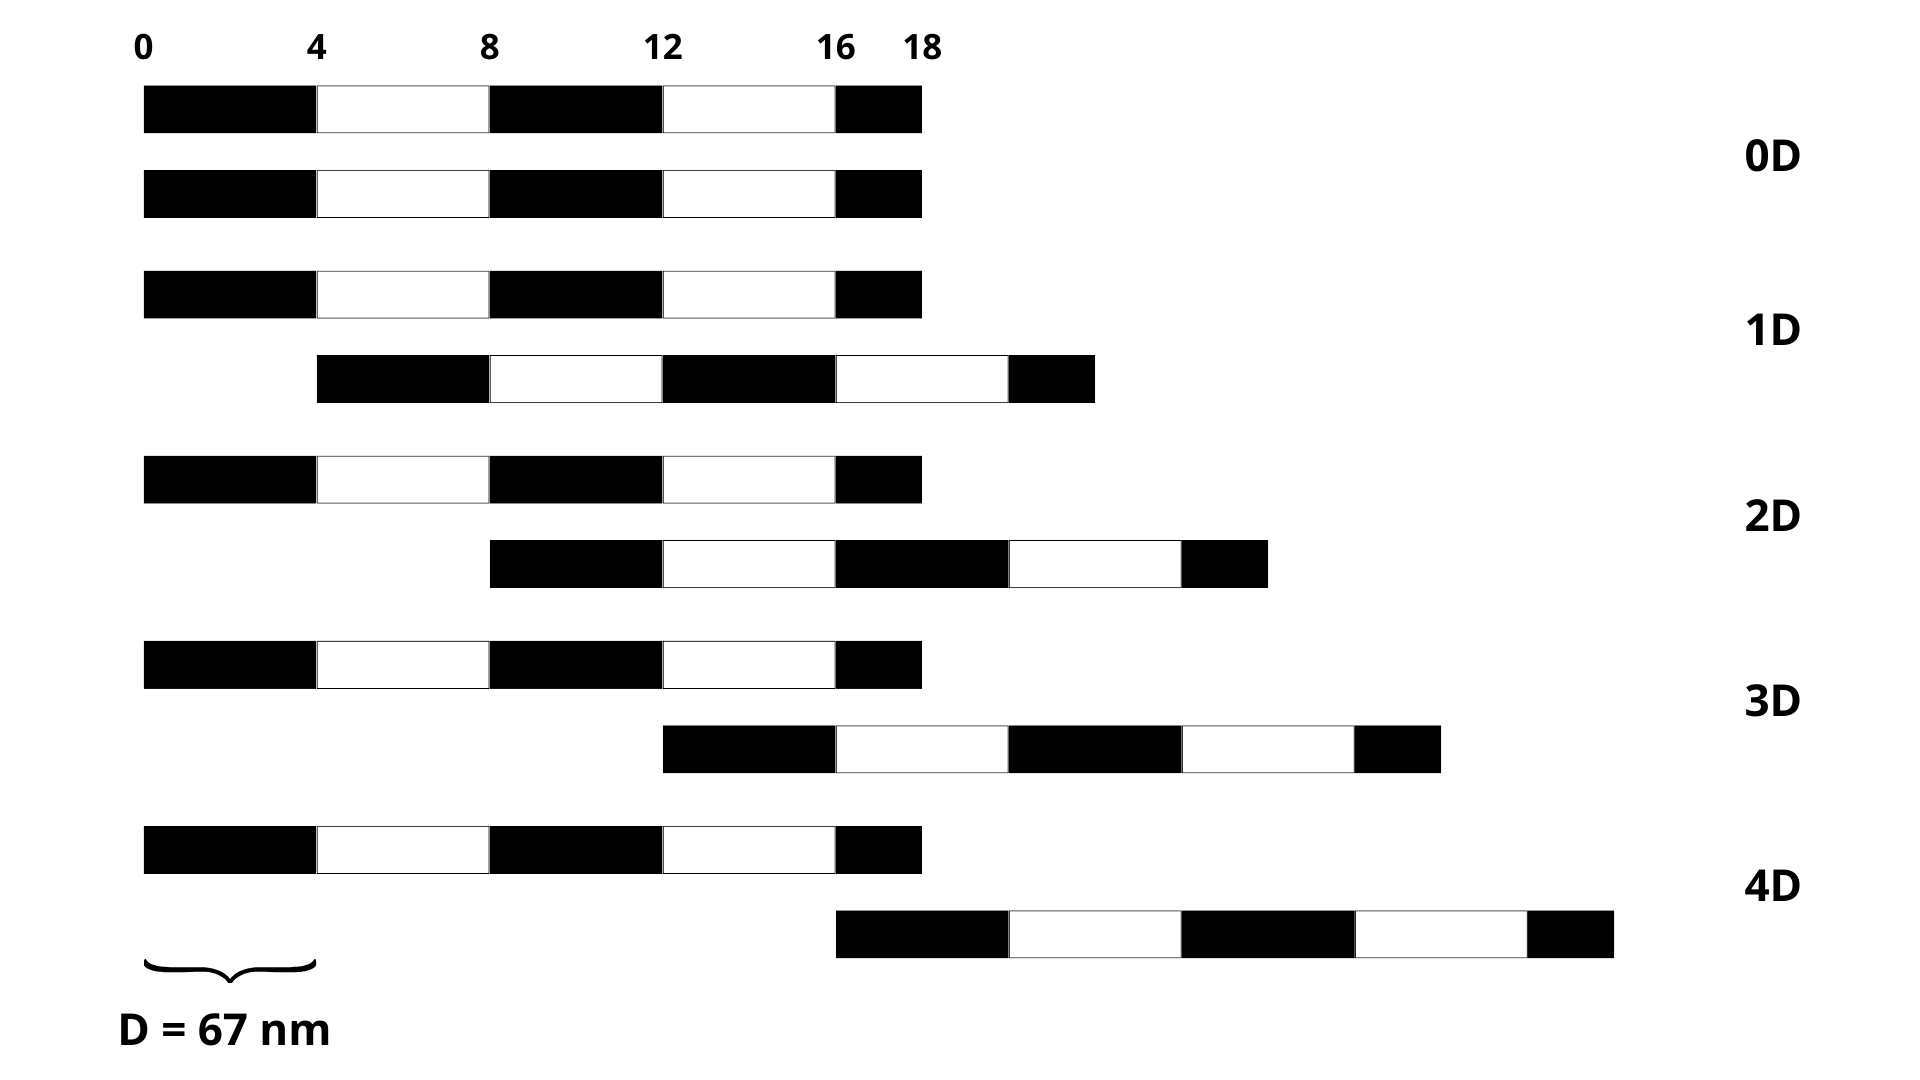
\includegraphics[width=\textwidth]{figures/specific_bind.png}
    
            \caption{Em fibrilas reais, observa-se que as moléculas estão alinhadas de forma escalonada, com um espaçamento característico de 
            \(D = 67 \, \text{nm}\). Visando uma modelagem mais precisa do fenômeno, implementamos uma regra de agregação que reproduz esse 
            processo, na qual novas moléculas são capturadas pelo agregado apenas se conectarem em posições que são múltiplos de \(D = 4\). 
            Assim, resultam cinco configurações possíveis de agregação para as novas moléculas.}  
    
            \label{M2}
        \end{figure}

        A formação de fibrilas reais é impulsionada por forças hidrofóbicas resultantes das interações entre as moléculas, as quais buscam 
        minimizar sua superfície exposta \cite{Kadler1987,Parkinson1995}. Para simular esse fenômeno, empregamos um algoritmo de difusão lateral
        na superfície, permitindo que uma molécula recém-agregada explore a superfície, mantendo sua coordenada \(y\) fixa, a fim de localizar 
        uma posição que minimize sua superfície exposta \cite{GarcaRuiz1991}. Em situações onde mais de uma posição minimiza a superfície, a 
        molécula permanece na primeira posição encontrada. Este mecanismo é regulado pelo parâmetro \(T_{s}\), que determina o número de 
        tentativas disponíveis para a molécula explorar a superfície do agregado \cite{Parkinson1995}.

        Com este algoritmo, geramos \(50\) fibrilas, cada uma contendo \(30.000\) bastões, para diferentes valores de \(T_{s}\), a fim de 
        investigar o efeito desse parâmetro na morfologia das fibrilas. 


    \subsection{Propriedades Mecânicas} 

        Para a análise das propriedades mecânicas das fibrilas, adotamos um modelo mecânico probabilístico. Esta abordagem é necessária, uma vez
        que os agregados gerados não apresentam propriedades elásticas adequadas para serem estudados por modelos baseados em molas, por exemplo
        \cite{Parkinson1997,Saitoh2020MolecularDS}.

        Primeiramente, realizamos o corte de um tronco de dimensão \(17 \times 201 \times 17\) em uma fibrila. Após este corte, procedemos com 
        uma limpeza para assegurar a ausência de moléculas desafixadas devido ao corte e para determinar o esqueleto ativo. Consideramos que o 
        tronco é composto por \(201\) camadas, e cada molécula, dividida em parcelas de tamanho unitário, pode estender-se por mais de uma camada.
        Iniciamos pela primeira camada, marcando todas as moléculas como ativas. Em seguida, verificamos nas camadas superiores se alguma 
        partícula de uma molécula ativa possui vizinhança inativa; caso afirmativo, a partícula é ativada, assim como todas as partículas 
        associadas à mesma molécula, tanto acima quanto abaixo. Este procedimento é repetido até alcançarmos a última camada, conforme ilustrado 
        na Figura \ref{M3}. Com essa seleção de moléculas ativas, repetimos o processo agora de cima para baixo até obtermos o esqueleto ativo, 
        que é o conjunto de moléculas através do qual uma força aplicada pode percolar. 

        \begin{figure}[H]
            \centering
            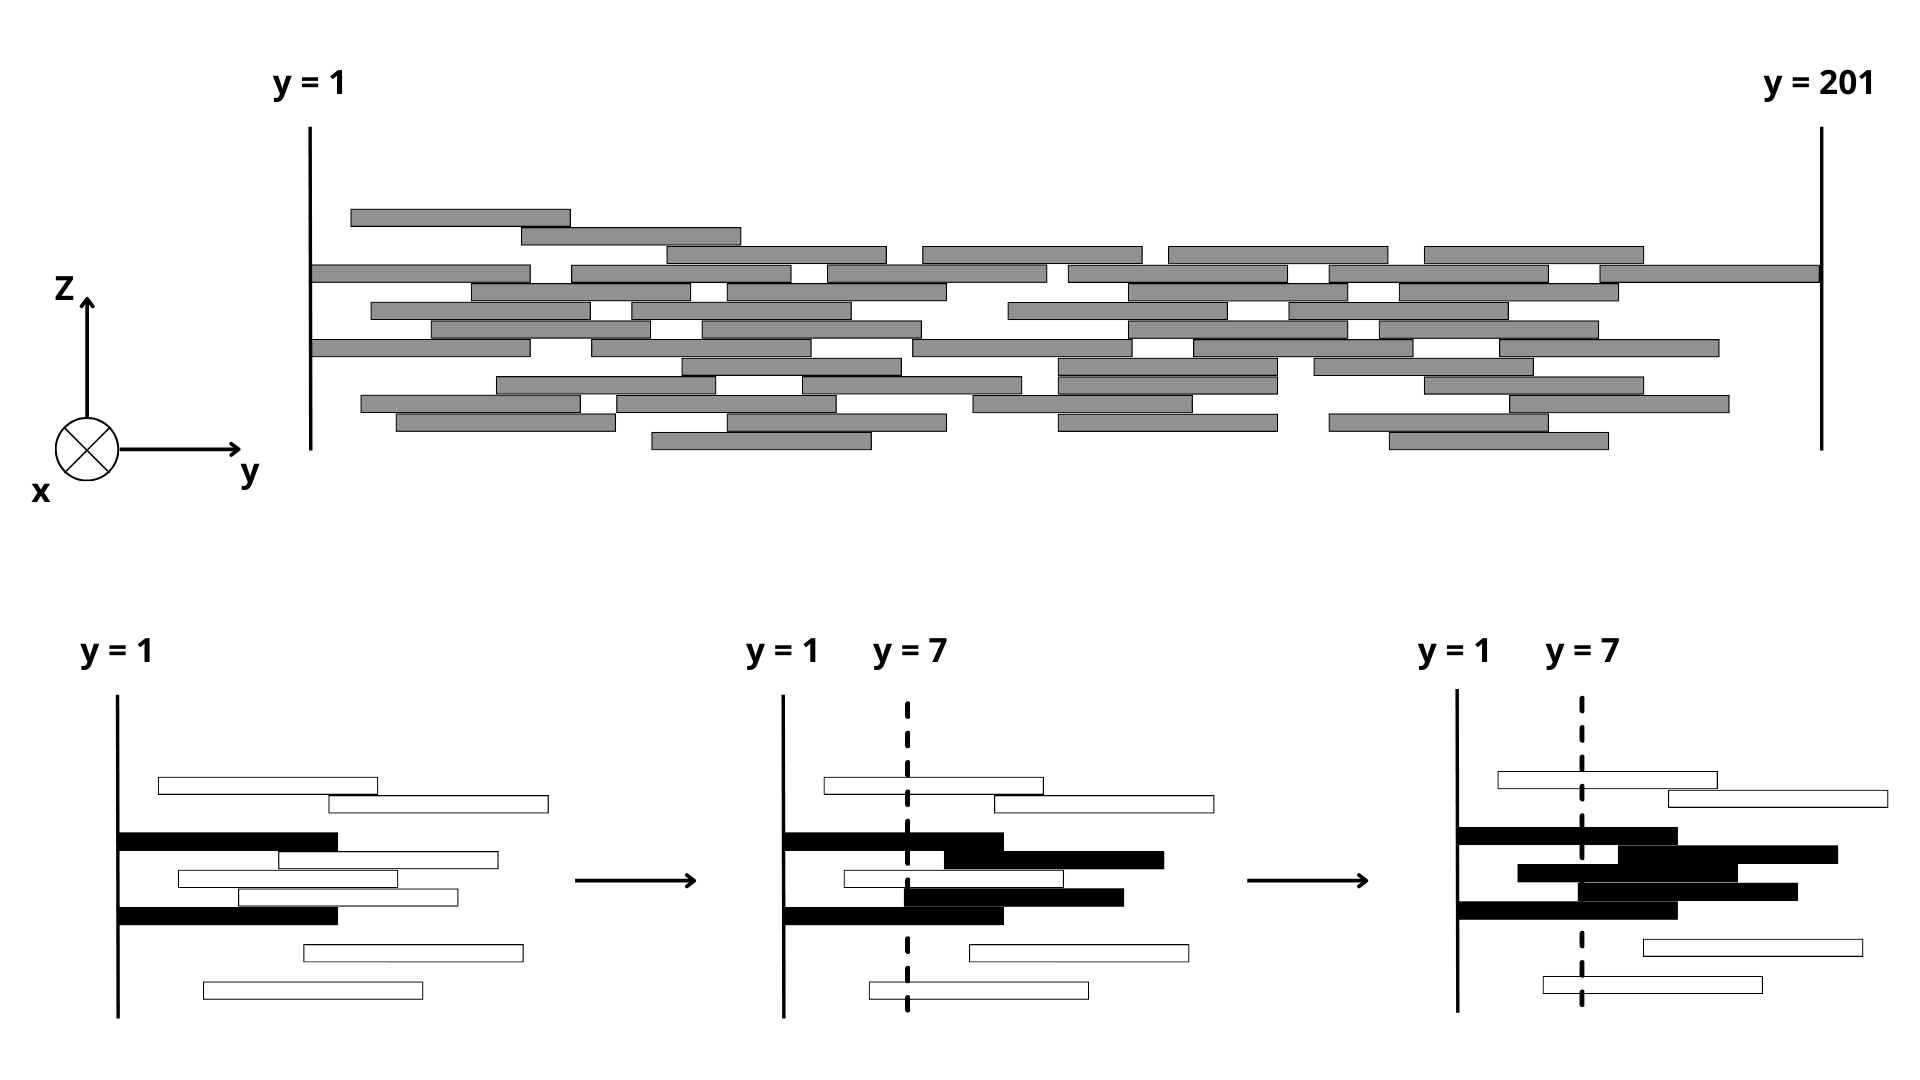
\includegraphics[width=\textwidth]{figures/esqueleto.png}
    
            \caption{A) Para análise das fibrilas, realizamos inicialmente o corte de um tronco com dimensões \(17 \times 201 \times 17\). B) 
            Procedemos com um processo de limpeza nesse tronco a fim de obter o esqueleto ativo, que efetivamente conduz a força na fibrila. 
            Iniciamos pela primeira camada do tronco, marcando como ativas todas as moléculas que possuem ao menos um segmento nesta camada. Em 
            seguida, avançamos para as camadas superiores e, para cada segmento ativo em uma dada camada, verificamos a existência de vizinhos 
            ativos. Caso existam, a molécula correspondente é marcada como ativa. Este procedimento é repetido até alcançarmos a última camada. 
            Com o conjunto de moléculas ativas identificado, as inativas são descartadas e o processo é então repetido, agora iniciando da 
            camada 201 e procedendo em direção à primeira camada.}  
    
            \label{M3}
        \end{figure}

        Após a determinação do esqueleto ativo, definimos para cada molécula uma probabilidade \(P_{R}\), influenciada tanto pela configuração de
        sua vizinhança quanto pela magnitude da força total aplicada ao agregado. Quando uma tensão é aplicada, cada molécula no agregado é 
        afetada por uma parcela dessa força total, proporcional ao número de partículas presentes em sua respectiva camada. Consequentemente, em 
        uma dada \(i\)-ésima camada contendo \(M\) partículas, a força por partícula é dada por:  

        \begin{equation}
            \sigma_{i} = \frac{F}{M_{i}},
        \end{equation}
            

        onde \(\sigma_{i}\) representa a força por partícula na \(i\)-ésima camada e \(F\) é a força total aplicada ao agregado. A força sentida 
        por uma molécula individual no agregado é, portanto, a média dos \(\sigma_{i}\) correspondentes às camadas em que a molécula está presente. 

        As moléculas de colágeno são caracterizadas por sua estrutura em tripla hélice \cite{BRODSKY1997545}, o que torna a ruptura intramolecular 
        menos provável em comparação com a quebra das ligações intermoleculares \cite{Parkinson1997}. Dessa forma, consideramos a probabilidade 
        de ruptura para a molécula como um todo, ao invés de para cada partícula individual que a compõe. Adicionalmente, assumimos que o número de 
        ligações responsáveis por manter a molécula fixada no esqueleto ativo é igual ao somatório do número de partículas vizinhas em cada camada 
        onde a molécula está presente. 

        Com base nesses pressupostos, definimos nossa probabilidade de ruptura pela equação 

        \begin{equation}
            P_{R} = \left(\frac{\langle \sigma_{i} \rangle}{N \sigma_{s}}\right)^{m},
        \end{equation}

        onde \(N\) representa o número de ligações de uma dada molécula, \(\sigma_{s}\) denota a força das ligações entre as moléculas, e \(m\) é um 
        fator que modula a dissipação de energia \cite{Parkinson1997,2013}. Em todas as simulações, adotamos \(m = 2\). 

        A simulação é conduzida aplicando-se uma força ao esqueleto ativo, em uma tentativa de emular os comportamentos observados em experimentos de 
        distensão. Inicialmente, calculamos a probabilidade de remoção \(P_{R}\) para cada molécula. Em seguida, realizamos um sorteio de um valor 
        entre 0 e 1 para cada molécula; se o valor sorteado for menor ou igual a \(P_{R}\), a molécula é removida. Este processo é repetido para 
        todas as moléculas do agregado. Após a primeira varredura, recalculamos \(P_{R}\) para as moléculas remanescentes sob a mesma força aplicada 
        e continuamos o processo até que não ocorram mais quebras. A força é então incrementada em meia unidade, e o procedimento é repetido. 
        Consideramos que a fibrila se rompe quando ao menos uma camada fica vazia, indicando que o esqueleto ativo não mais forma um agregado 
        percolante. Esse procedimento está esquematizado na Figura \ref{M4}. Monitoramos o processo de remoção das moléculas, registrando a quantidade 
        de moléculas removidas para uma dada força e a tensão máxima suportada antes da ruptura. 


        \begin{figure}[H]
            \centering
            \includegraphics[width=\textwidth]{figures/simulaçao (1).png}
    
            \caption{A) Com o esqueleto ativo definido, simulamos um teste mecânico na fibrila, análogo à aplicação de uma força axial ao longo do eixo 
            \(y\), estendendo-a. Dada a ausência de propriedades elásticas na fibrila, recorremos a um modelo mecânico probabilístico. Neste modelo, 
            atribuímos a cada molécula uma probabilidade de remoção \(P_{R}\), que depende tanto da força aplicada ao agregado quanto do número de 
            ligações que a molécula mantém. B) Iniciamos a simulação atribuindo \(P_{R}\) a cada molécula e sorteando uma probabilidade \(P_{i}\). Se 
            \(P_{i} \leq P_{R}\), a molécula é removida do agregado. Este processo é repetido até que todas as moléculas sejam avaliadas, seguido pelo 
            recálculo de \(P_{R}\) para as moléculas remanescentes. A força é incrementada em meio após cada ciclo no qual não ocorrem mais remoções. C) 
            A simulação termina quando identificamos uma camada vazia no agregado, momento no qual consideramos a fibrila como rompida.} 
    
            \label{M4}
        \end{figure}

      
        Consideramos a quantidade de moléculas rompidas como um indicador da deformação da nossa fibrila. Além disso, determinamos a tensão em relação 
        às forças calculadas para aproximar a simulação a uma fibrila real. A força necessária para romper uma ligação é considerada constante, e 
        utilizamos o diâmetro médio das fibrilas para calcular a tensão. 

        Para cada valor de \(T_{s}\), selecionamos 10 fibrilas para submeter ao procedimento de simulação. Para cada fibrila, realizamos mil experimentos. 
        Registramos, para cada nível de força aplicada, o número de moléculas removidas do esqueleto e quantas permaneceram. 
        


\section{Resultados}
    \subsection{Morfologia das fibrilas}

    Os agregados gerados pelo modelo apresentam uma morfologia fibrilar, com características relevantes de sua forma 
    sendo determinadas pelo parâmetro \(T_{s}\). Podemos observar, na Figura \ref{R1}, a estrutura desses agregados 
    para os valores de \(T_{s} = 2\), baixa difusão, e \(T_{s} = 10000\), alta difusão lateral sobre a superfície. As 
    fibrilas com menor \(T_{s}\) apresentam uma forma mais aberta, enquanto para valores mais altos, observamos uma 
    forma mais compacta e regular. A coloração indica o quão antiga uma molécula é no agregado, indo do azul escuro, 
    mais antigas, para o amarelo, mais recentes. Nos agregados mais compactos, temos dificuldade em observar moléculas
    mais antigas visto que essas estão muito no interior da estrutura. Para as mais abertas, temos uma maior facilidade
    em observar moléculas mais antigas. Além disso, na visão lateral, observamos o comportamento alongado e com pontas 
    afinadas, típico de fibrilas reais. 

    \begin{figure}[H]
        \centering
        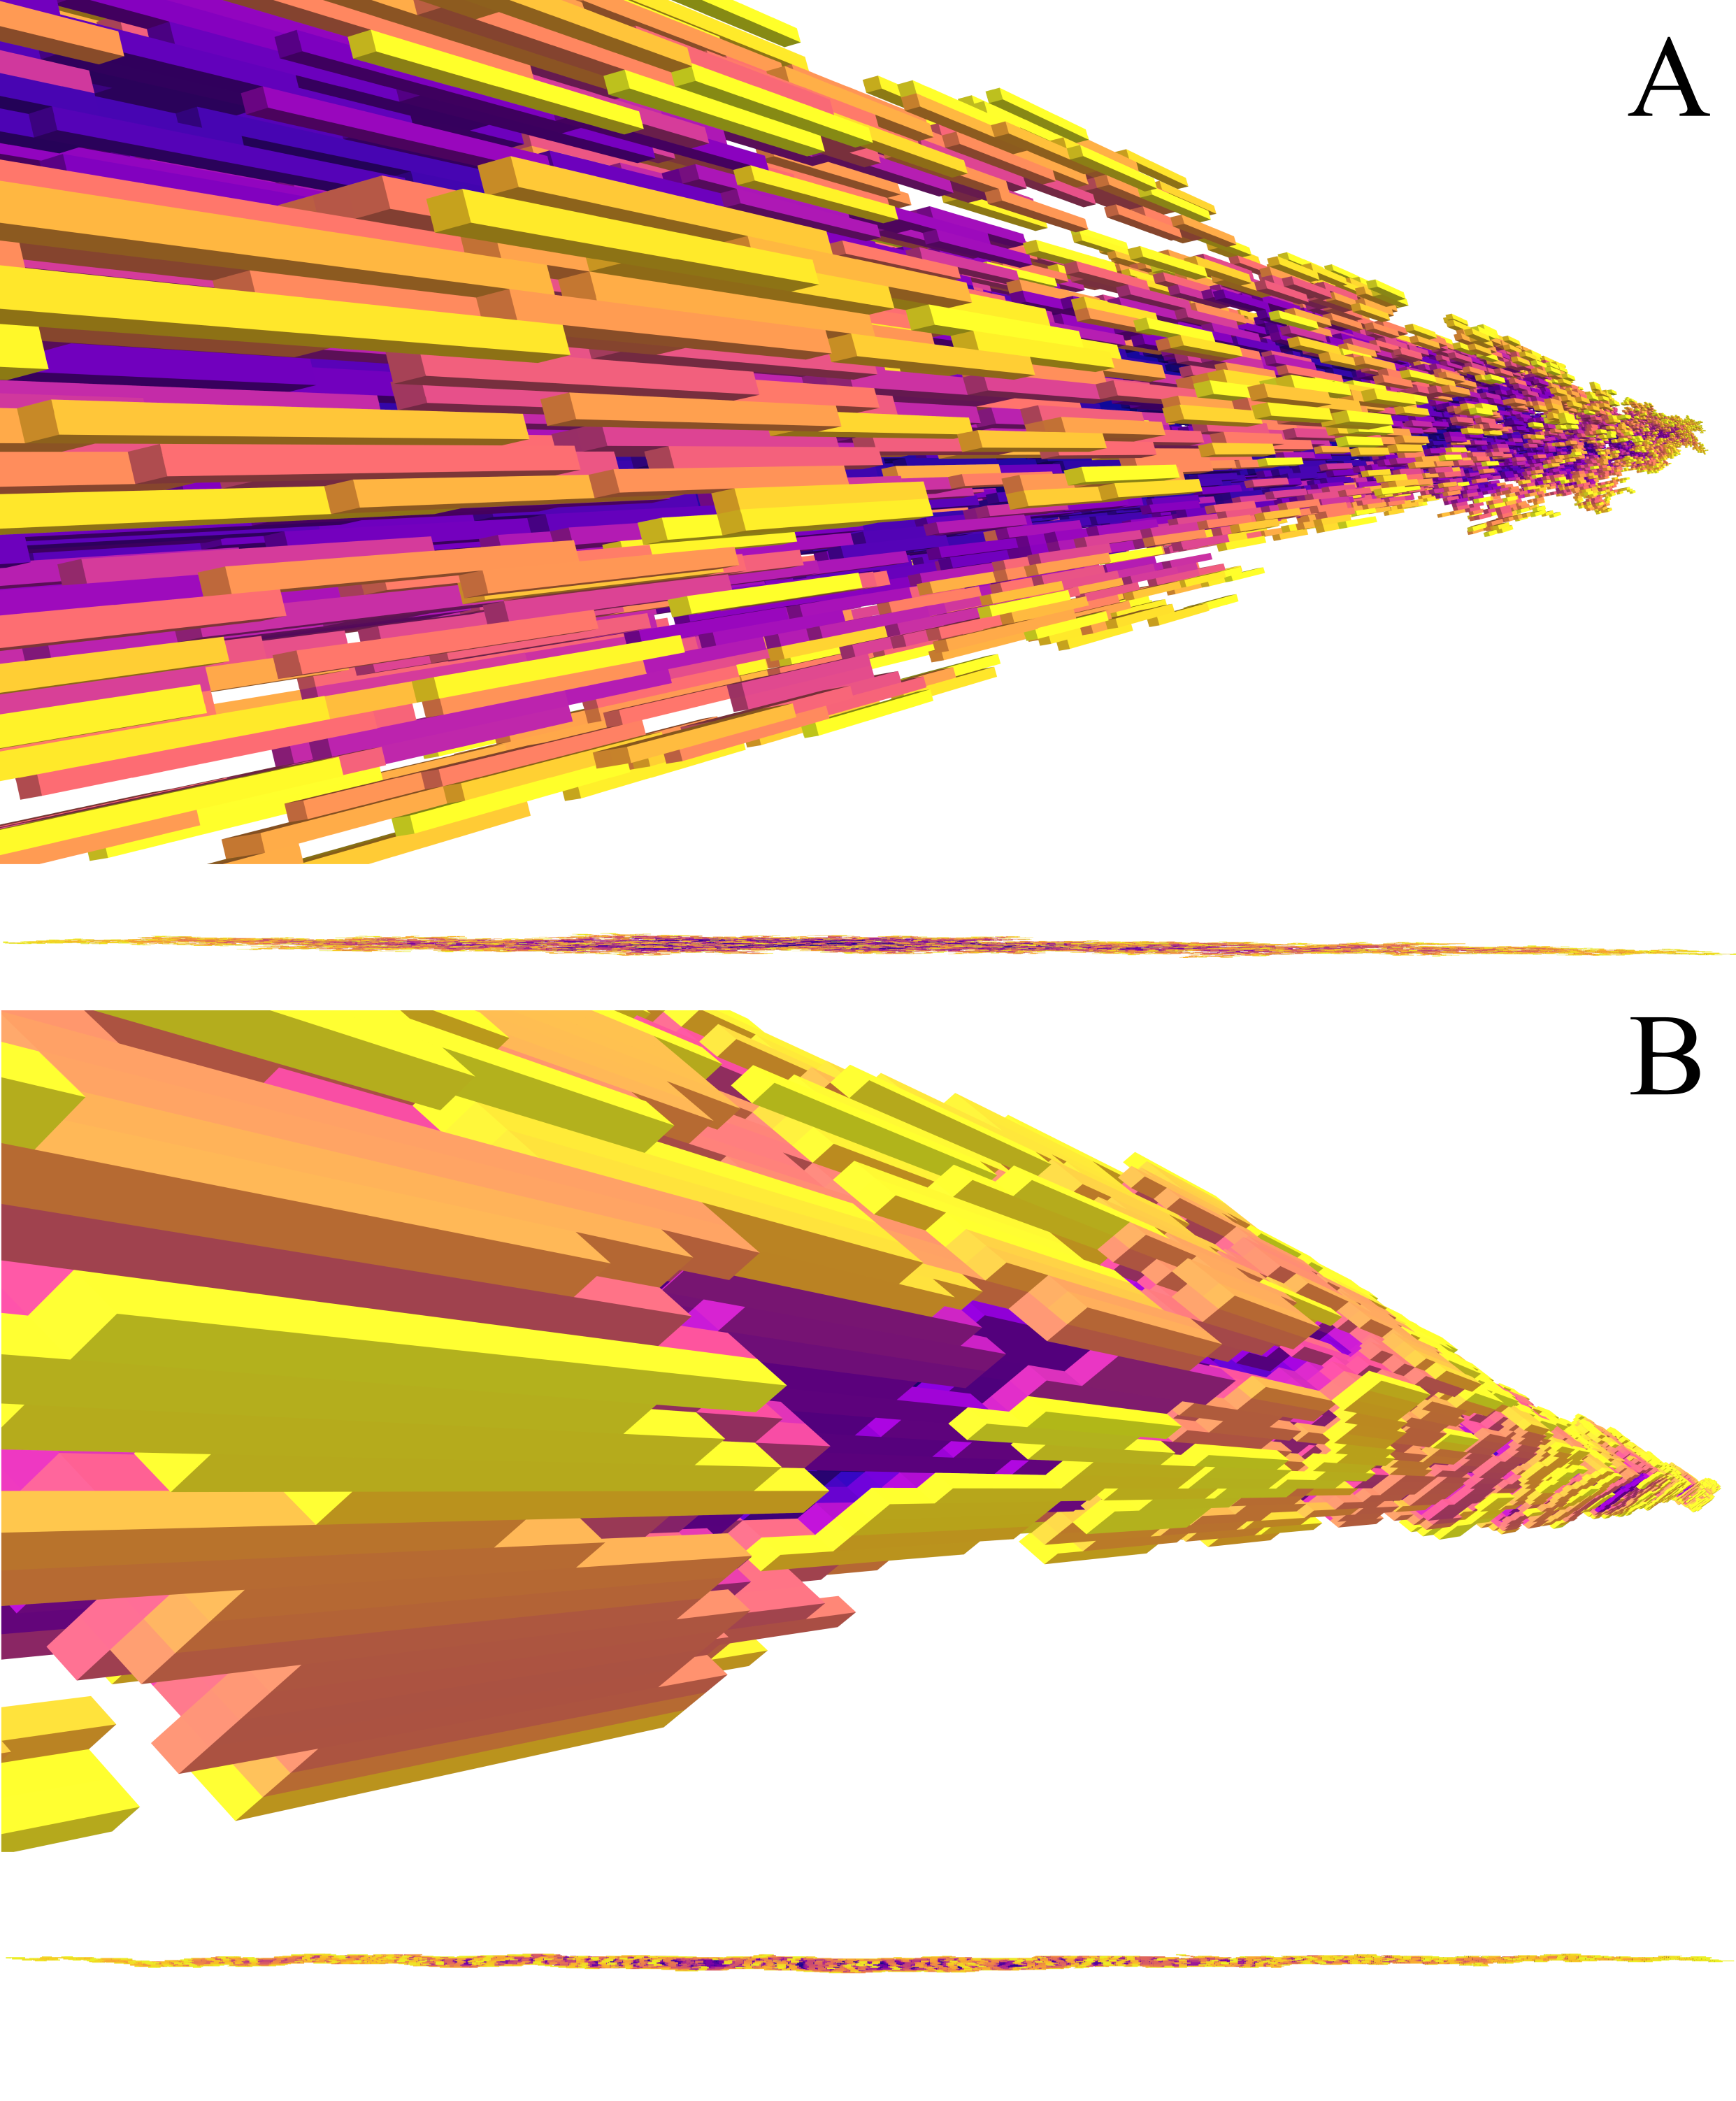
\includegraphics[width=\textwidth]{figures/fibrils.png}

        \caption{Visualização transversal e lateral das fibrilas geradas com o algoritmo de DLA contendo 30.000 moléculas.
        A coloração indica quão antigo é a molécula no agregado. Quanto mais pro azul escuro, 
        mais antigo no agregado, quanto mais para o amarelo, mais recente. 
        A) Fibrila gerada para \(T_{s}\) 2, baixa difusão. B) Fibrila gerada para \(T_{s}\) = 10000, alta difusão.} 

        \label{R1}
    \end{figure}

    O comprimento, o diâmetro e a densidade da região central das fibrilas são características influenciadas pelo 
    parâmetro \(T_{s}\). Na Tabela \ref{tab1}, podemos observar como essas dimensões se alteram, em média, com o 
    aumento desse parâmetro. O comprimento e a densidade tendem a aumentar com o incremento de \(T_{s}\), enquanto 
    o diâmetro tende a diminuir. Uma propriedade comum a essas medidas é que elas exibem um comportamento de 
    estabilização à medida que nos aproximamos de \(T_{s} = 512\); a partir desse ponto, elas oscilam em torno de um 
    valor médio. 

    \begin{table}[H]
        \caption{Valores médios dos comprimentos, diametros e densidade de fibrilas geradas para diferentes valores de \(T_{s}\).}

        \centering  % Mantém a tabela centralizada no texto
        \begin{tabular}{lccc}
        \hline
        \textbf{$T_{s}$} & \multicolumn{1}{c}{\textbf{Length(u.m)}} & \textbf{Ray(u.m)} & \textbf{Density(\% )} \\ \hline
        2                & 3668.36                                   & 32.40             & 0.17                  \\
        8                & 3695.16                                   & 28.68             & 0.25                  \\
        16               & 3764.27                                   & 24.63             & 0.34                  \\
        32               & 3808.68                                   & 21.67             & 0.46                  \\
        64               & 3891.56                                   & 17.6              & 0.57                  \\
        128              & 3928.6                                    & 16.06             & 0.62                  \\
        512              & 3913.24                                   & 14.07             & 0.66                  \\
        1024             & 3912.52                                   & 14.14             & 0.65                  \\
        4096             & 3892.28                                   & 14.06             & 0.66                  \\
        8192             & 3892.52                                   & 14.16             & 0.66                  \\
        10000            & 3917.16                                   & 13.94             & 0.65                  \\ \hline
        \multicolumn{1}{l}{Limit Upper} & 3905.54                    & 14.08             & 0.65                  \\ \hline
        \end{tabular}
        \label{tab1}  % Substitua 'meu_rótulo' pelo rótulo desejado para a referência cruzada
    \end{table}


    Outra característica desses agregados é a relação linear entre a massa e a distância até as pontas. Na Figura 
    \ref{R2}, observamos que, independentemente do valor de \(T_{s}\), todos os agregados exibem esse comportamento. 
    Tal característica é recorrentemente observada tanto em fibrilas reais quanto nas simuladas com este modelo 
    \cite{Parkinson1995,Kadler1987}. 


    \begin{figure}[H]
        \centering
        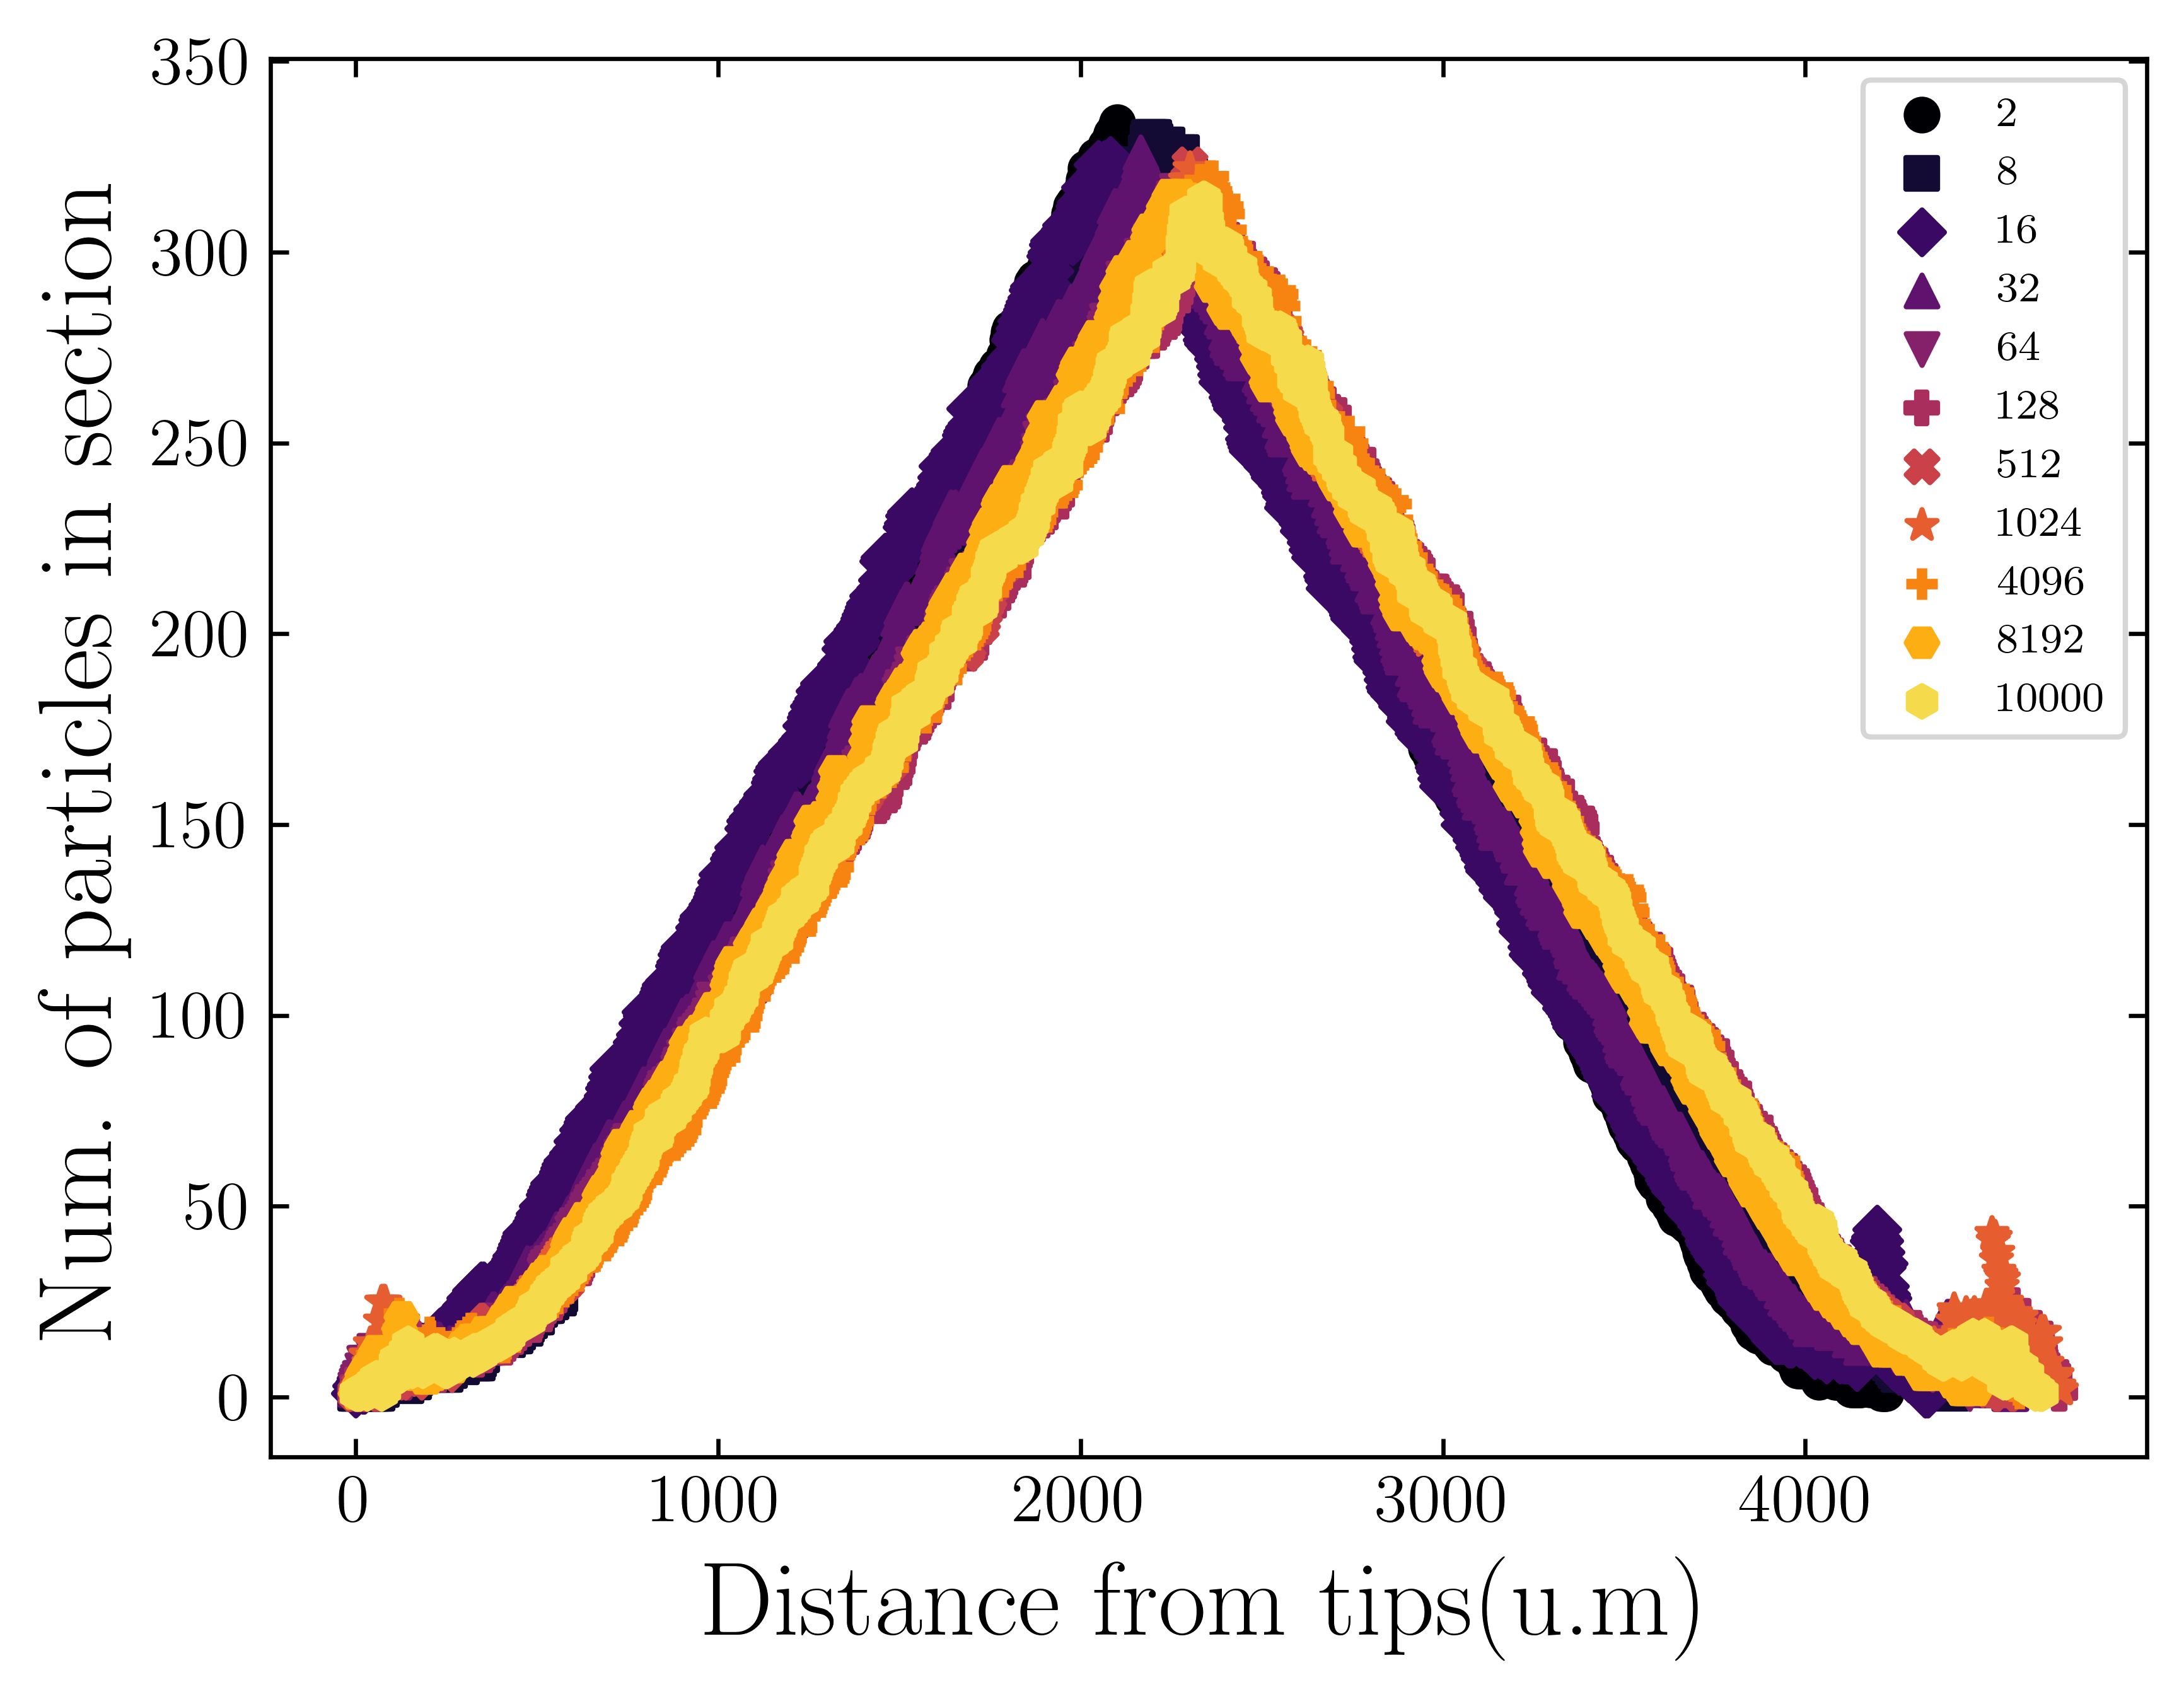
\includegraphics[width=\textwidth]{figures/tips.png}

        \caption{A quantidade de partículas por seção das fibrilas geradas segue uma relação linear da distancia em que 
        medimos para a ponta. Nos observamos que, partindo de uma ponta, a massa cresce linear até bem proximo da região
        central da fibrila. A medida que nos afastamos dessa região, a massa decaí linearmente. Esse comportamento foi 
        observado para todas as fibrilas, indicando que o parâmetro \(T_{s}\) não tem efeito sobre essa característica.} 

        \label{R2}
    \end{figure}


    Analisando a seção transversal das fibrilas, conforme ilustrado na Figura \ref{R3}, observamos que o aumento do 
    parâmetro \(T_{s}\) resulta na diminuição dos espaços vazios dentro da seção, levando à formação de agregados mais 
    compactos e quase completamente preenchidos. Devido a essa característica progressiva em função do parâmetro 
    \(T_{s}\), calculamos a dimensão fractal das seções e constatamos que, à medida que \(T_{s}\) aumenta, ocorre um 
    incremento no valor médio da dimensão fractal da seção até atingir uma saturação. Na Figura \ref{R4}, é evidente 
    que para valores mais baixos de \(T_{s}\), a dimensionalidade é próxima da observada em agregados gerados pelo 
    modelo de Agregação Limitada por Difusão (DLA) \cite{Witten1983}, que é de 1.71, remetendo ao nosso modelo de 
    formação. Enquanto isso, para valores mais elevados de \(T_{s}\), a dimensão fractal tende a estabilizar em valores 
    próximos a 1.93, que se assemelha muito à dimensão euclidiana para objetos bidimensionais. 

    \begin{figure}[H]
        \centering
        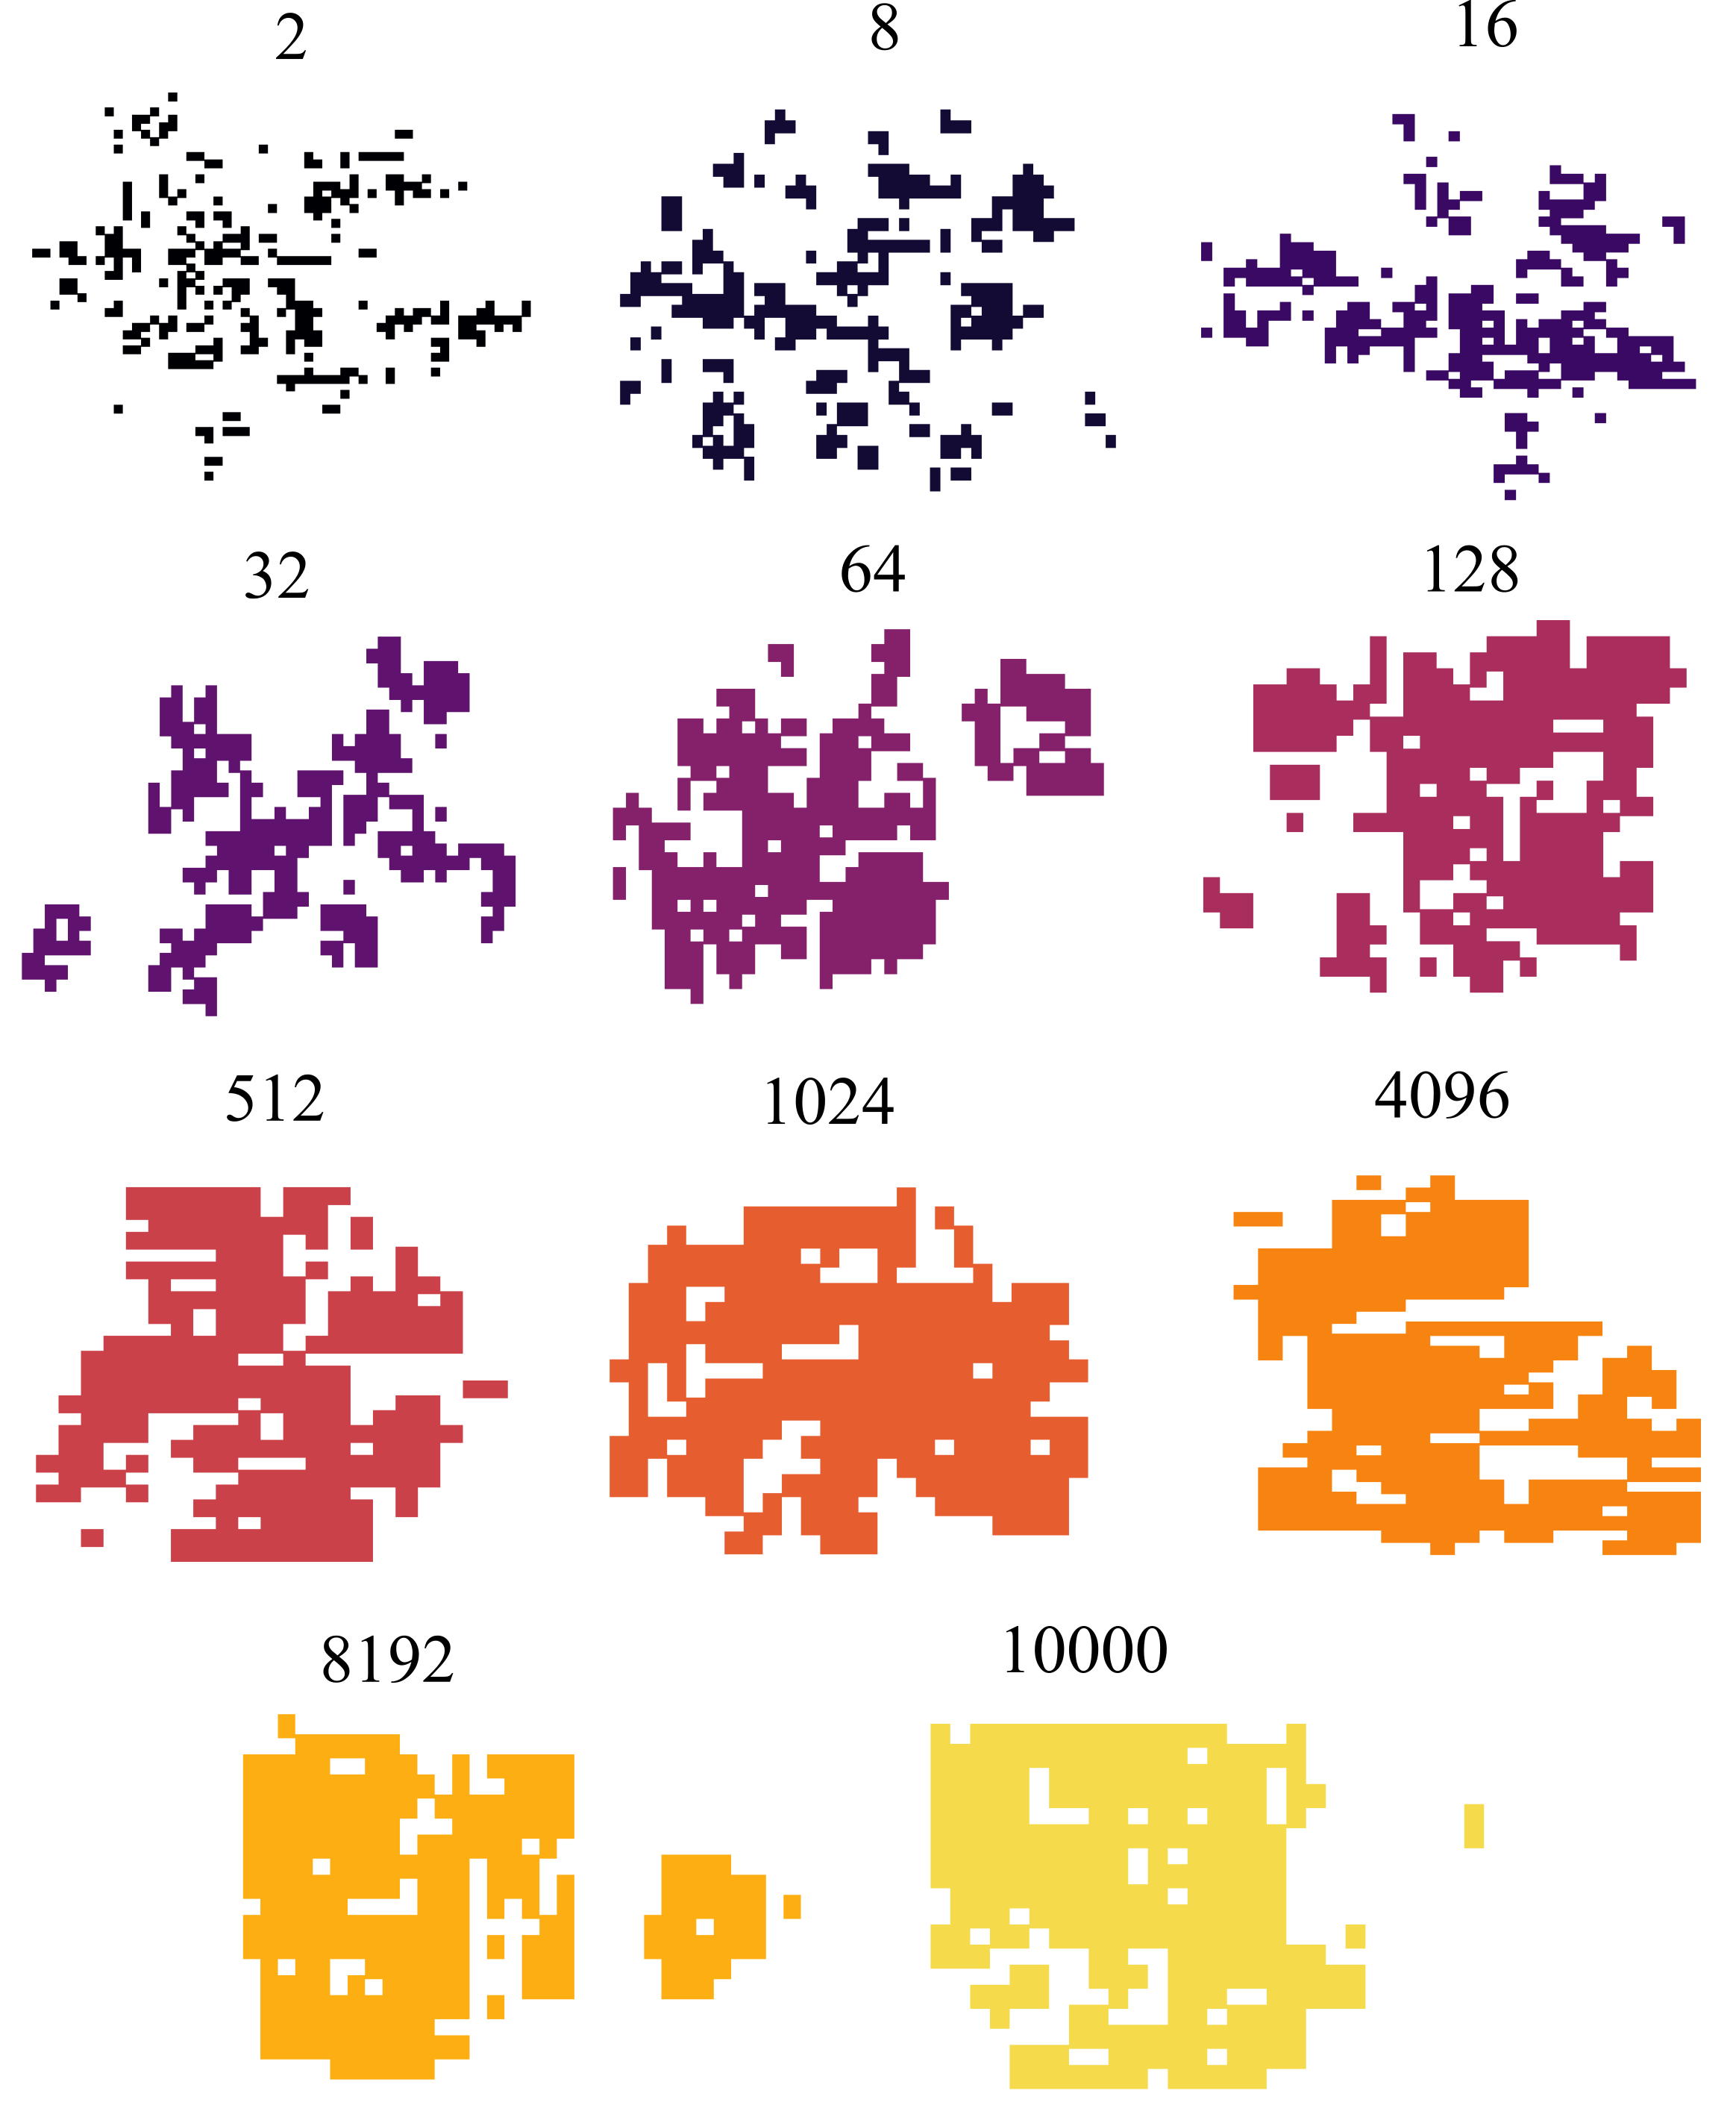
\includegraphics[width=\textwidth]{figures/cs_all.png}
        \caption{Variação da forma da seção transversal das fibrilas para diferentes valores de \(T_{s}\).} 
        \label{R3}
    \end{figure}

    \begin{figure}[H]
        \centering
        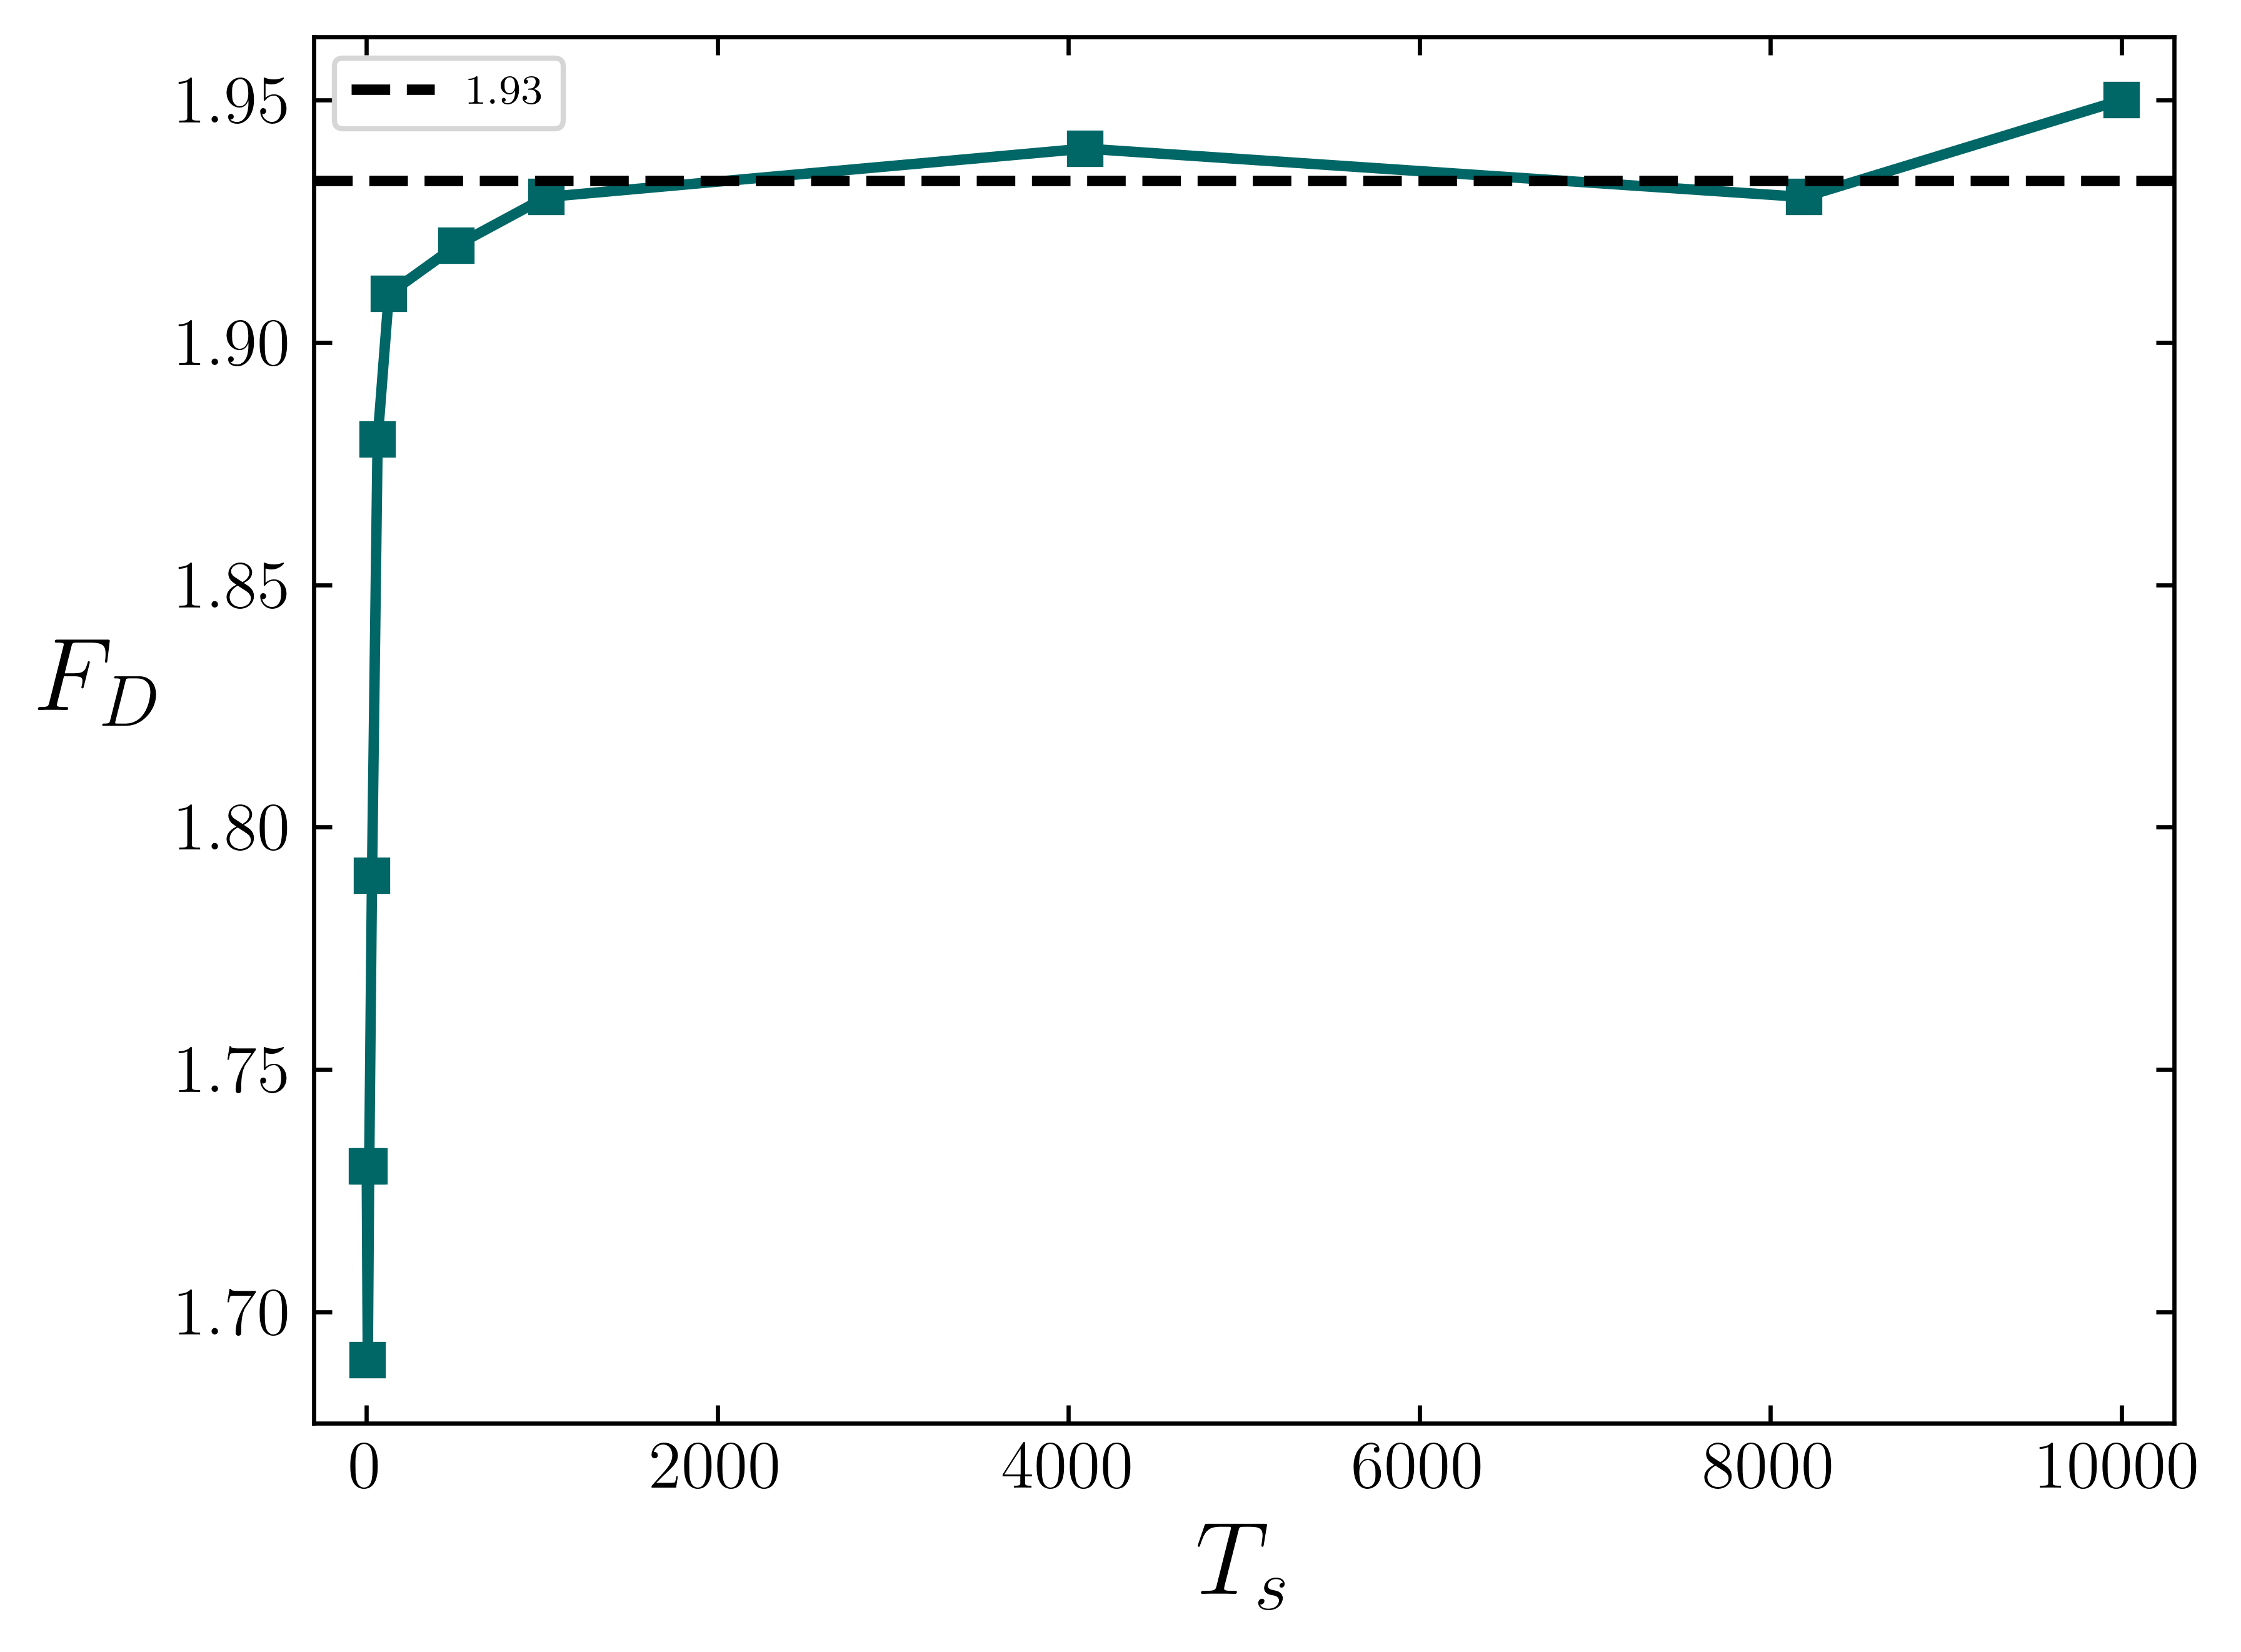
\includegraphics[width=\textwidth]{figures/dim_frac.png}

        \caption{ Dimensão fractal média da sesção transversal em função do parâmetro \(T_{s}\).} 

        \label{R4}
    \end{figure}


    \subsection{Propriedades mecânicas}

    Para compreender como nosso agregado responde à aplicação de uma força axial, avaliamos como o número de 
    moléculas na fibrila varia com a força. Na Figura \ref{R5}, apresentamos a curva de stress-strain para agregados 
    gerados com diferentes valores de \(T_{s}\). Observamos que o aumento desse parâmetro influencia no incremento da 
    tensão máxima de ruptura. No entanto, a partir de \(T_{s} = 512\), esses valores se tornam bastante próximos e as 
    curvas começam a se sobrepor. Comumente, esperaríamos que essas curvas crescessem de forma mais abrupta até o valor
    máximo, o que não é observado aqui. Esse comportamento mais suave até o valor limite é uma consequência do módulo 
    de Weibull que utilizamos no modelo. Para valores baixos, a curva resultante é não determinística 
    \cite{Parkinson1997}. A tensão máxima suportada que encontramos foi de 45,6 MPa, valor muito próximo ao encontrado 
    por Yang et al. \cite{YANG2012148} ao analisar fibrilas reconstituídas do tendão de Aquiles bovino purificado. 
    Em contraste, no trabalho de Yamamoto \cite{Noritaka}, foram utilizadas fibrilas isoladas do fascículo dos tendões 
    da cauda de ratos, obtendo um valor de 100 \(\pm\) 32 MPa. A discrepância em relação ao nosso valor pode estar 
    associada à dimensão das fibrilas utilizadas por ele, que apresentavam um diâmetro significativamente maior do que 
    as modeladas neste trabalho.

    \begin{figure}[H]
        \centering
        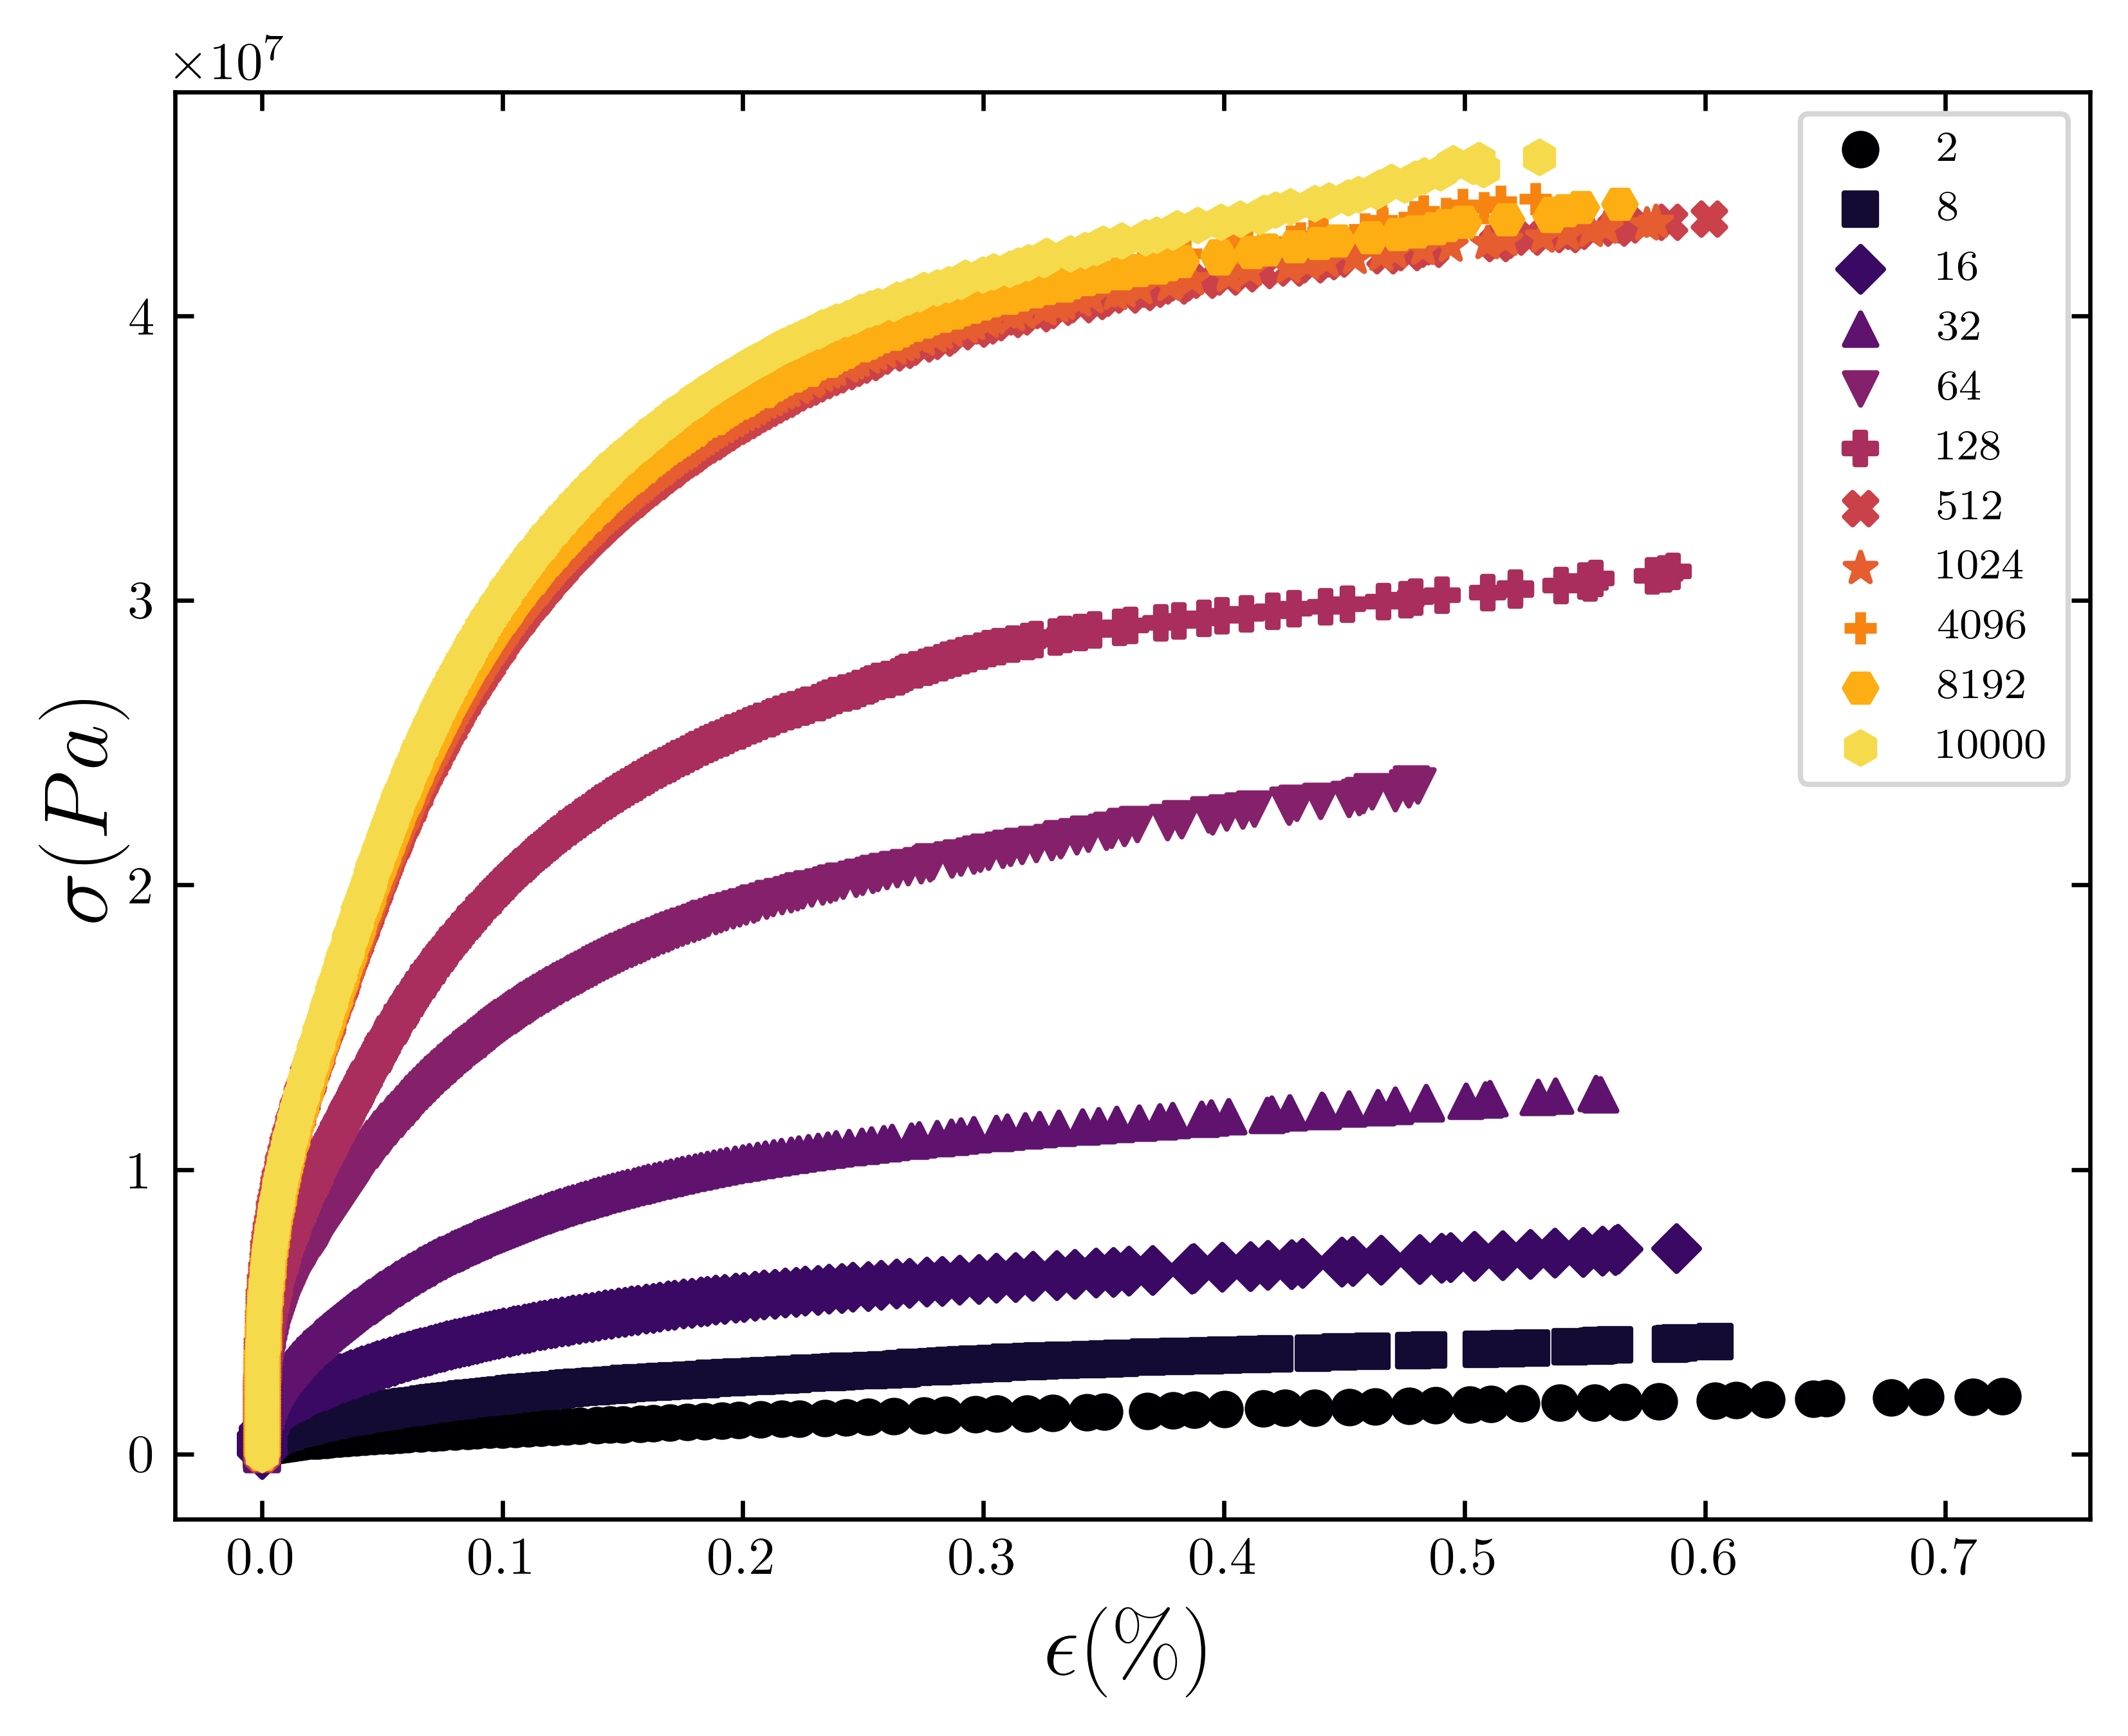
\includegraphics[width=\textwidth]{figures/stress_strain.png}

        \caption{Tensão em função da deformação da fibrila para diferentes valores de \(T_{s}\).} 

        \label{R5}
    \end{figure}

    Na Figura \ref{R6}, podemos observar como os valores de tensão máxima suportada variam com um parâmetro 
    importante das fibrilas, a densidade. Escolhemos essa análise visto que o comportamento de \(\sigma\) e da 
    densidade, \(\rho\), exibem formas semelhantes quando analisados em função de \(T_{s}\). Identificamos um 
    comportamento exponencial no aumento da tensão máxima até um limite superior de 44,1 MPa. A saturação da 
    densidade ocorre em 65\%, valor este próximo ao encontrado por Parkinson et al.\cite{Parkinson1995} com esse 
    modelo, porém um pouco abaixo do determinado por Katz et al.\cite{KATZ1973351}, que calculou experimentalmente 
    cerca de 80\% do espaço disponível ocupado para as fibrilas de colágeno. Com base nessa característica de 
    saturação, consideramos que, dado o custo computacional elevado, este modelo pode ser executado, para os parâmetros 
    que inicialmente utilizamos, com \(T_{s}=512\), uma vez que nesse ponto já obtemos fibrilas com os valores de 
    interesse médios equivalentes para valores superiores desse parâmetro. 



    \begin{figure}[H]
        \centering
        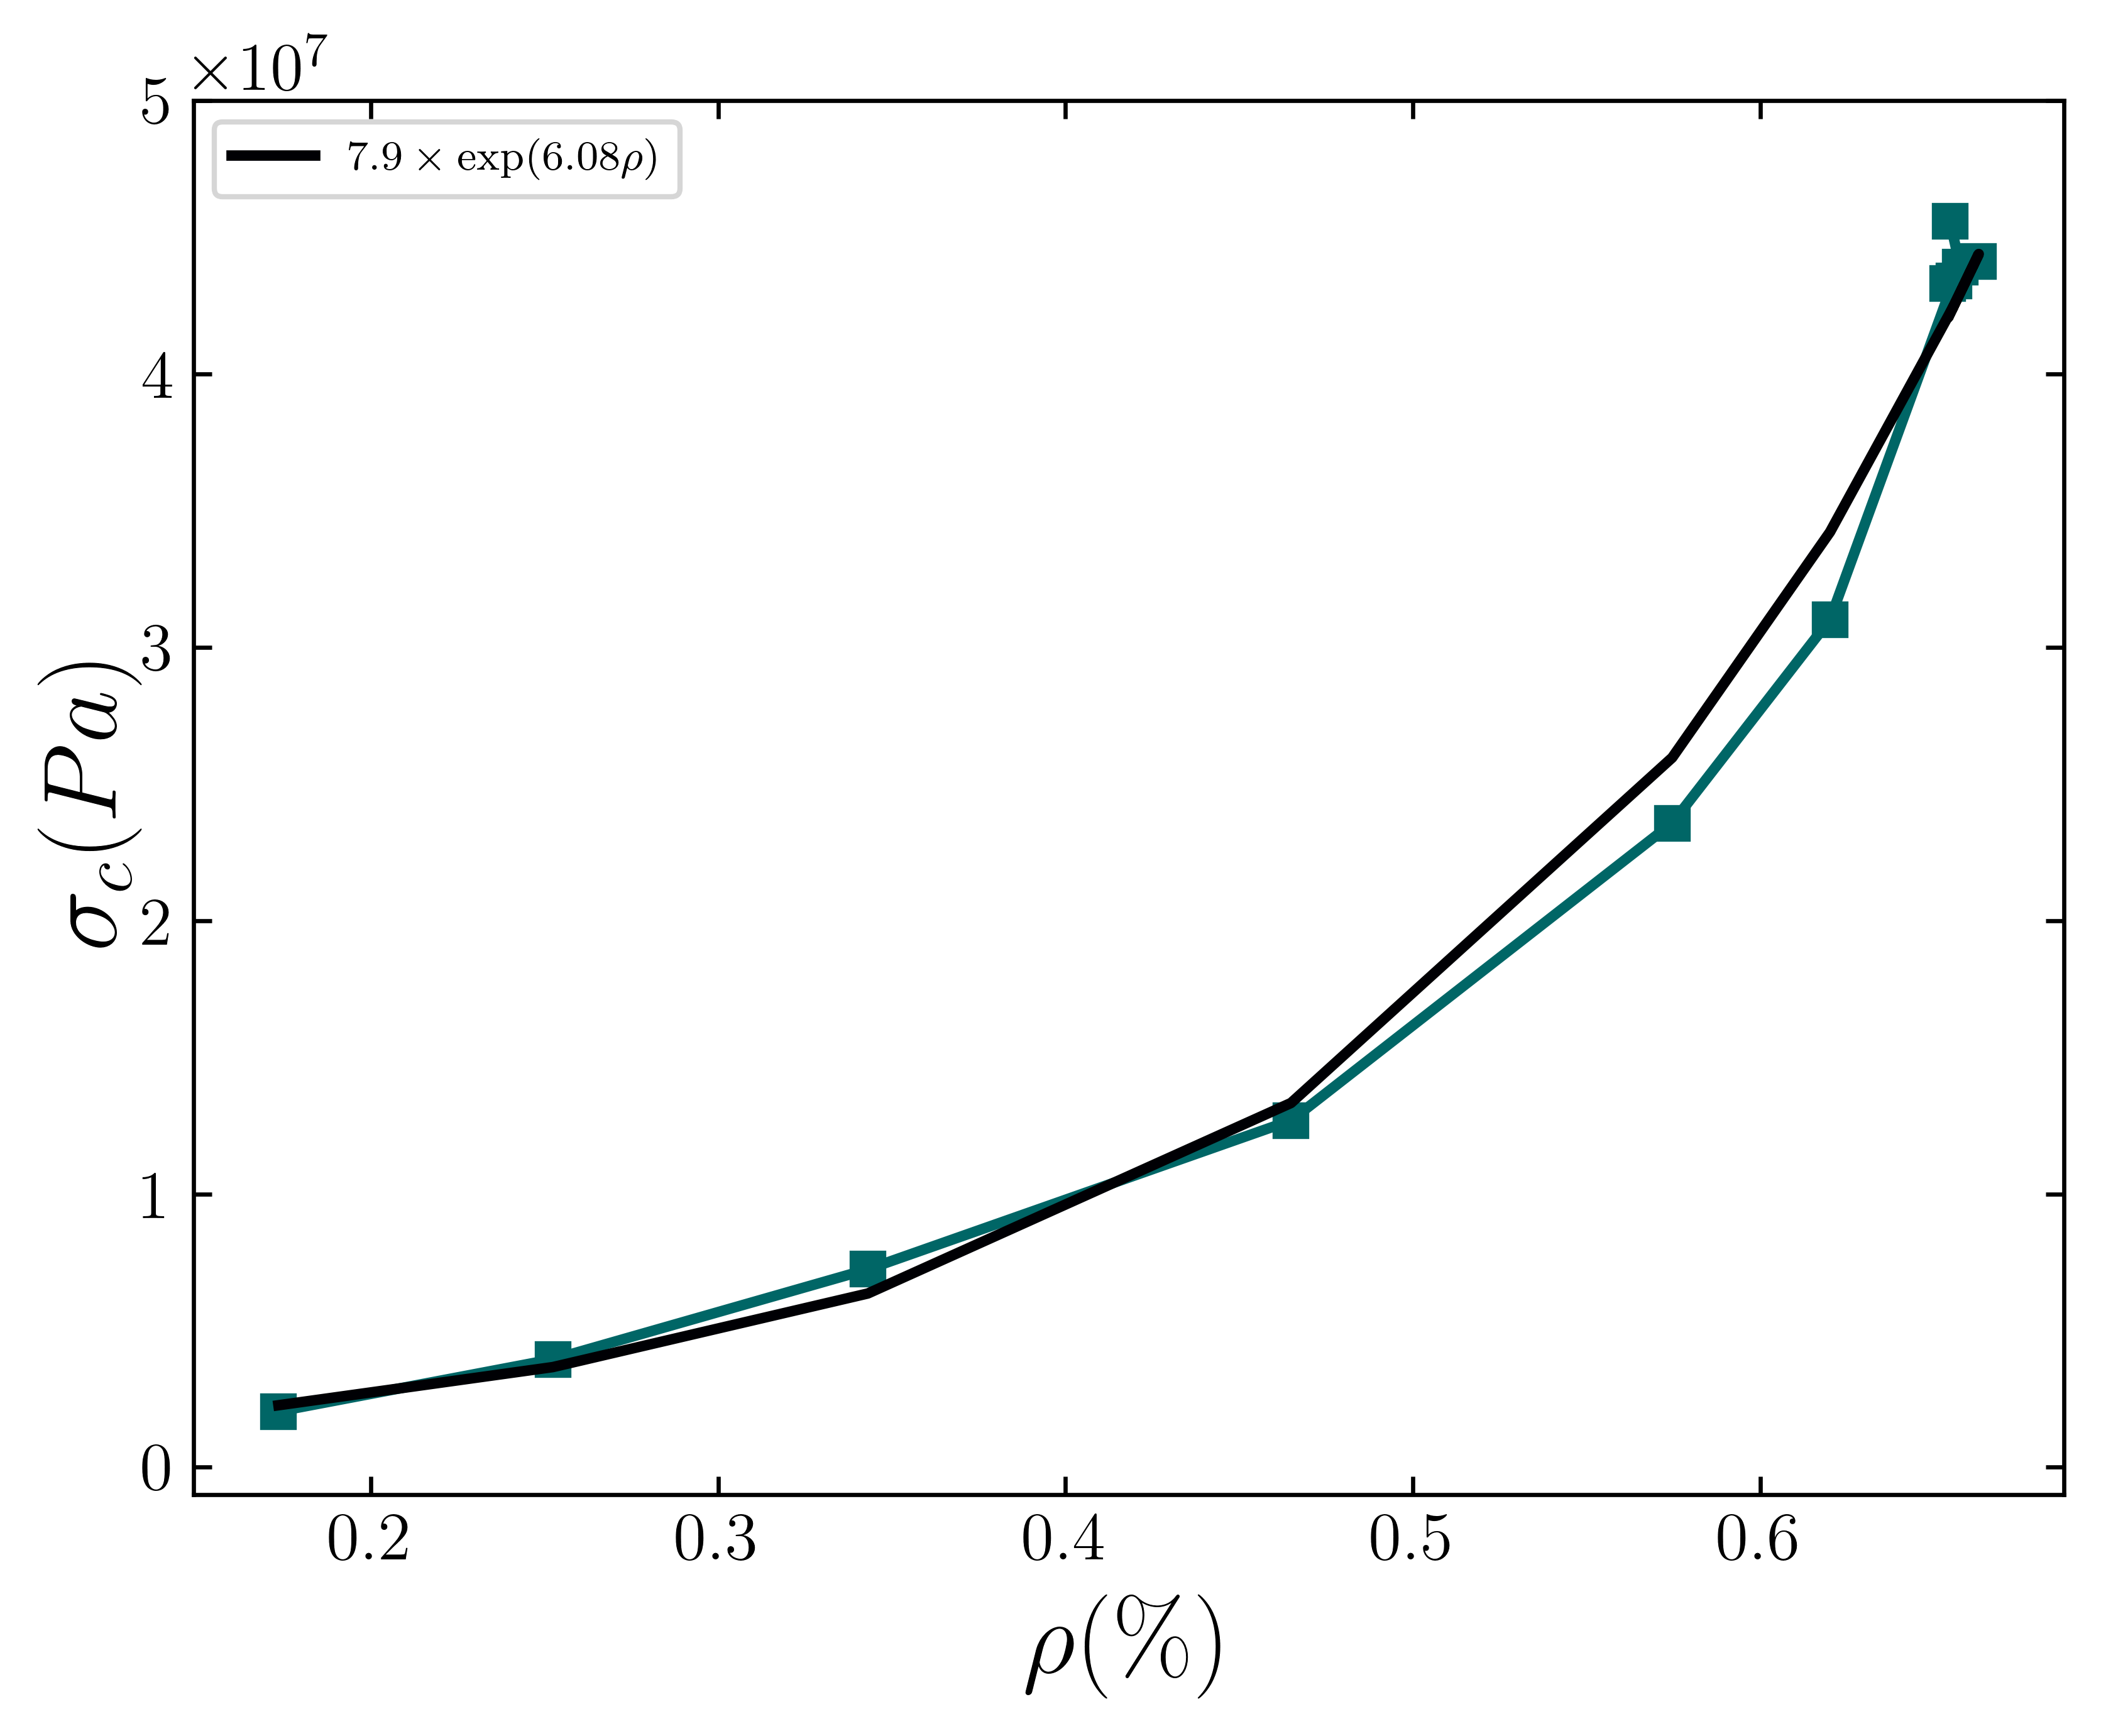
\includegraphics[width=\textwidth]{figures/sigma_rho.png}

        \caption{Tensão crítica em função da densidade. Observamos que esse valor cresce exponencialmente com a 
        densidade até ambos os parâmetros atingirem um limite superior.} 


        \label{R6}
    \end{figure}

    Ao analisar como o processo de ruptura ocorre no nosso modelo, bem como em outros, constatamos que a 
    redistribuição de tensão, para uma mesma força, pode levar à ocorrência de rupturas em cascata. Na Figura 
    \ref{R7}, apresentamos a distribuição das avalanches de ruptura em função do seu tamanho. É possível observar a 
    existência de duas ordens de grandeza bem definidas; após isso, os dados são afetados pelo efeito de tamanho 
    finito. Analisando a região de interesse, até próximo de \(10^{2.5}\), conseguimos determinar o expoente das leis 
    de escala de modo que eles aumentam com o crescimento de \(T_{s}\). Este comportamento é compreensível ao 
    considerarmos que a densidade aumenta com este parâmetro, resultando em mais moléculas para contribuir com os 
    tamanhos das avalanches. Assim, temos que as avalanches durante o processo de ruptura são independentes do tamanho 
    do sistema; contudo, elas são influenciadas pelo quão compacta é a fibrila, com o expoente \(\gamma\) variando de 
    -1.94 até -2.60. 


    \begin{figure}[H]
        \centering
        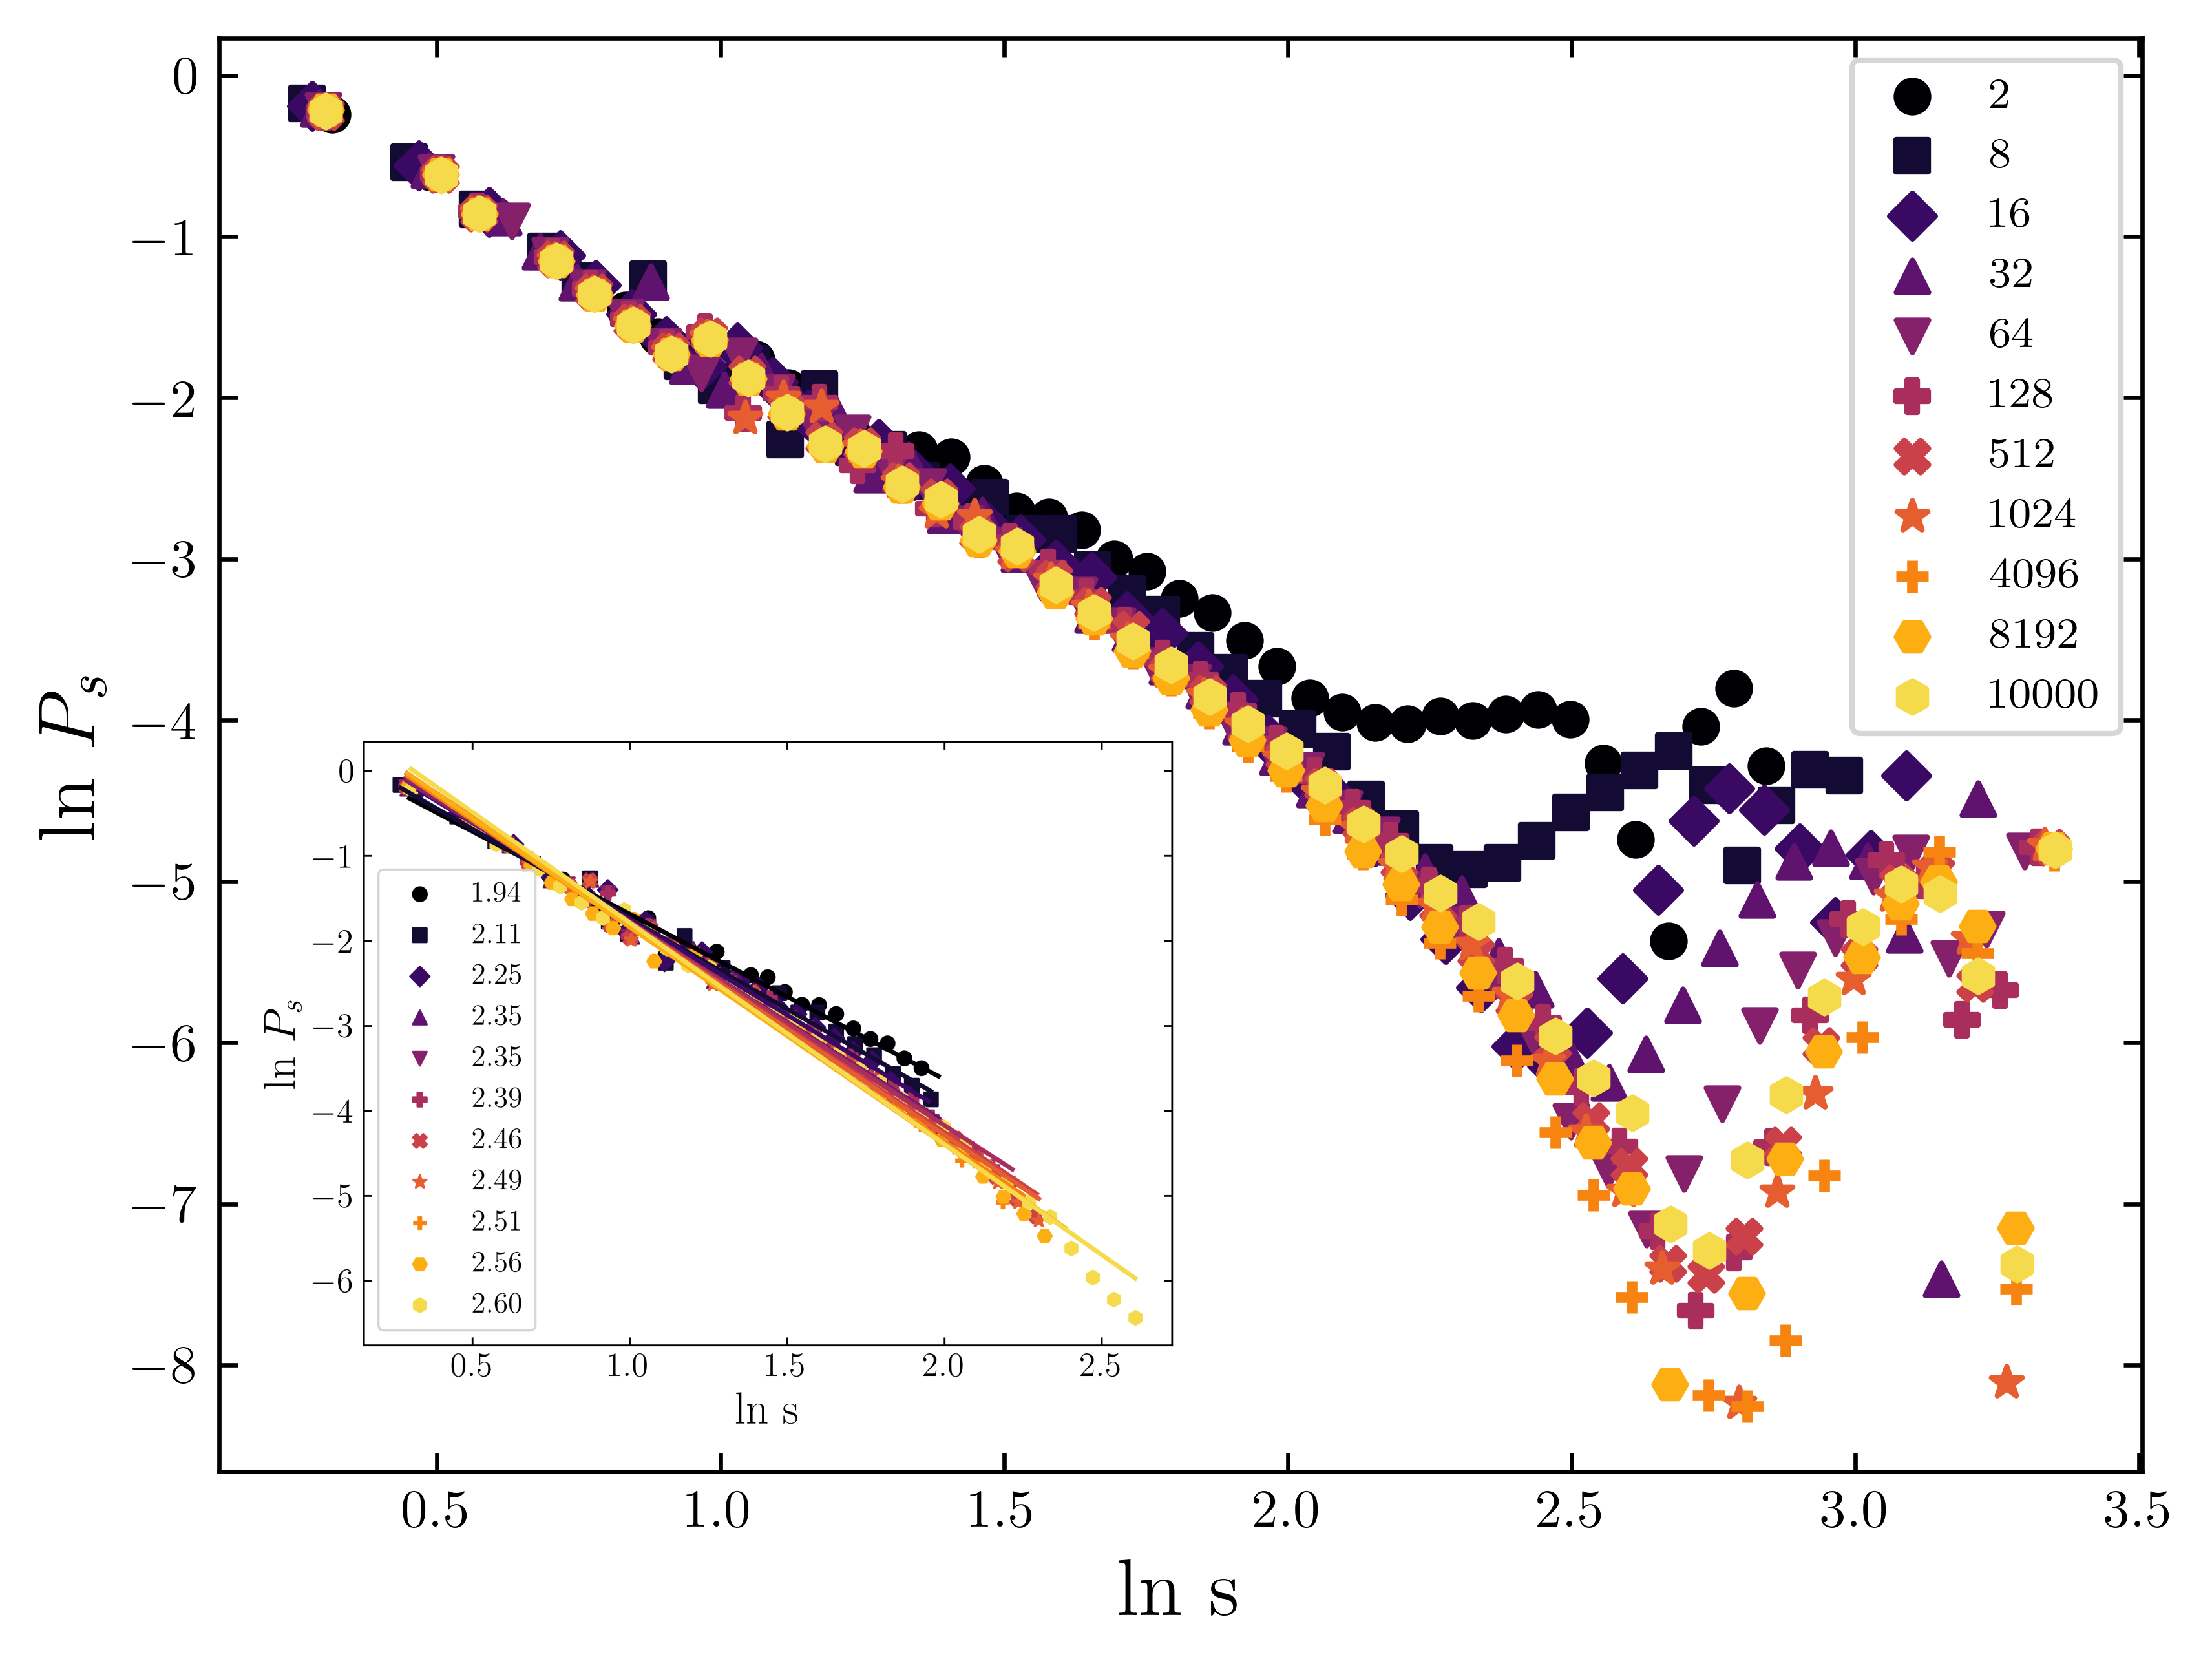
\includegraphics[width=\textwidth]{figures/ava.png}

        \caption{Distribuição das avalanches de ruptura em função do seu tamanho para diferentes valores de \(T_{s}\).
        Podemos observar um comportamento em lei de potencia com expoentes $\gamma$ bem definidos para todos valores do 
        parâmetro. Os expoentes variam de -1.94 a -2.60.} 

        \label{R7}

    \end{figure}

\section{Conclusões}

    Neste estudo, demonstramos a capacidade de um modelo baseado em Agregação Limitada por Difusão (DLA) com difusão 
    superficial para simular a formação de fibrilas de colágeno, resultando em agregados com características morfológicas 
    semelhantes às das fibrilas reais. O parâmetro \(T_{s}\) mostrou-se cruciail para definir várias propriedades das 
    fibrilas, como comprimento, densidade e diâmetro, que tendem a variar de maneira inversamente proporcional a \(T_{s}\). 
    Observou-se uma relação linear entre a massa das fibrilas e a distância até as pontas, além de uma variação na dimensão 
    fractal da seção central, que aumenta com \(T_{s}\), variando de 1.71 a 1.93.

    A resistência máxima à tensão das fibrilas aumenta com \(T_{s}\), alcançando um limite de 44,1 MPa, e a tensão crítica 
    suportada apresenta uma correlação exponencial com a densidade das fibrilas. O processo de ruptura revelou avalanches 
    de ruptura com leis de potência definidas, cujos expoentes variam de -1.94 a -2.60, indicando que, embora as avalanches 
    sejam independentes do tamanho do sistema, elas são influenciadas pela compactação da fibrila.

    Essas descobertas sugerem que as fibrilas geradas pelo modelo apresentam uma tensão máxima suportada que aumenta com a 
    densidade e com \(T_{s}\). Fibrilas mais resistentes tendem a ter uma dimensão fractal mais próxima da dimensão 
    euclidiana de objetos bidimensionais e exibem valores mais elevados no expoente das leis de potência. Além disso, muitas 
    das propriedades analisadas tendem a saturar, indicando que simulações realizadas com \(T_{s} = 512\) são suficientes para 
    observar os valores máximos de interesse, otimizando o uso de recursos computacionais.






\bibliographystyle{unsrtnat} % Set the bibliography style
\bibliography{ref.bib} % Include your .bib file (without the .bib extension)


    
\end{document}
